% options:
% thesis=B bachelor's thesis
% thesis=M master's thesis
% czech thesis in Czech language
% slovak thesis in Slovak language
% english thesis in English language
% hidelinks remove colour boxes around hyperlinks

\documentclass[thesis=B,czech]{FITthesis}[2012/06/26]

\usepackage[utf8]{inputenc}
\usepackage{float}
\usepackage{multirow}
% \usepackage[unicode]{hyperref}
\usepackage{listings}
\usepackage{color}


\RequirePackage{pdfpages}


\definecolor{dkgreen}{rgb}{0,0.6,0}
\definecolor{gray}{rgb}{0.5,0.5,0.5}
\definecolor{mauve}{rgb}{0.58,0,0.82}

\lstset{frame=tb,
  language=Java,
  aboveskip=3mm,
  belowskip=3mm,
  showstringspaces=false,
  columns=flexible,
  basicstyle={\small\ttfamily},
  numberstyle=\tiny\color{gray},
  keywordstyle=\color{blue},
  commentstyle=\color{dkgreen},
  stringstyle=\color{mauve},
  breaklines=true,
  breakatwhitespace=true,
  tabsize=3,
  numbers=left
}

\lstdefinelanguage{JavaScript}{
  keywords={typeof, new, true, false, catch, function, return, null, catch, switch, var, if, in, while, do, else, case, break},
  keywordstyle=\color{blue}\bfseries,
  ndkeywords={class, export, boolean, throw, implements, import, this},
  ndkeywordstyle=\color{darkgray}\bfseries,
  identifierstyle=\color{black},
  sensitive=false,
  comment=[l]{//},
  morecomment=[s]{/*}{*/},
  commentstyle=\color{purple}\ttfamily,
  stringstyle=\color{red}\ttfamily,
  morestring=[b]',
  morestring=[b]"
}

\usepackage{graphicx} %graphics files inclusion
% \usepackage{amsmath} %advanced maths
% \usepackage{amssymb} %additional math symbols

\usepackage{dirtree} %directory tree visualisation

% % list of acronyms
% \usepackage[acronym,nonumberlist,toc,numberedsection=autolabel]{glossaries}
% \iflanguage{czech}{\renewcommand*{\acronymname}{Seznam pou{\v z}it{\' y}ch zkratek}}{}
% \makeglossaries

\newcommand{\tg}{\mathop{\mathrm{tg}}} %cesky tangens
\newcommand{\cotg}{\mathop{\mathrm{cotg}}} %cesky cotangens


% % % % % % % % % % % % % % % % % % % % % % % % % % % % % % 
% ODTUD DAL VSE ZMENTE
% % % % % % % % % % % % % % % % % % % % % % % % % % % % % % 

\department{Katedra \ldots (softwarového inženýrství)}
\title{ InfoWeb - Nástroj získávání informací z webů }
\authorGN{Jakub} %(křestní) jméno (jména) autora
\authorFN{Tuček} %příjmení autora
\authorWithDegrees{} %jméno autora včetně současných akademických titulů
\supervisor{Ing. Jiří Hunka}
\acknowledgements{Rád bych poděkoval za trpělivost vedoucímu Ing. Jiřímu Hunkovi, rodině za podporu a svému týmu
z předmětů BI-SP1 a BI-SP2 za obětavou práci na společném projektu.}

\abstractCS{
Tato práce rozebírá problematiku získávání informací z webů s důrazem na potřeby internetových obchodů jako například vývoj ceny produktu
u konkurence.
Jelikož této práci předcházel týmový projekt z předmětů BI-SP1 a BI-SP2 je popsaná i daná týmová realizace včetně zvolených postupů. 
Po zhodnocení týmového řešení jsou navrženy možné změny, které
doplňují funkcionalitu, umožňují lepší rozšiřitelnost a opravují nežádoucí chování systému.
Výsledkem práce je refaktoring týmového řešení spolu s rozšířením o nejdůležitější vylepšení. Vzniklý systém je na základě důkladného otestování znova zhodnocen. Finálně jsou navržena další vylepšení pro budoucnost projektu.
}
\abstractEN{
This thesis describes difficulties of data mining from web with emphasis on the needs of online shops. Such need is for example trend of product prices sold by competitors. Because this issue was already addressed in team project implemented in courses BI-SP1 and BI-SP2, thesis describes created system, including chosen work methods.
After analysis of created team project, possible changes are designed. These changes are extending existing functionality, improving expandability and fixing unwanted behaviour of created system.
Goal of thesis is refactoring of team project along with implementing most important changes. Created system is evaluated based on thorough 
testing. Finally, additional improvements are designed for possible future system usage.
}
\placeForDeclarationOfAuthenticity{V~Praze}
\declarationOfAuthenticityOption{4} %volba Prohlášení (číslo 1-6)
\keywordsCS{informace z webu, internetové obchody, cena produktu, Git, Jenkins, průběžná integrace, modulární architektura}
\keywordsEN{data mining, online shopping, product price, Git, Jenkins, Continuous Integration, Modular Architecture}

\begin{document}

% \newacronym{CVUT}{{\v C}VUT}{{\v C}esk{\' e} vysok{\' e} u{\v c}en{\' i} technick{\' e} v Praze}
% \newacronym{FIT}{FIT}{Fakulta informa{\v c}n{\' i}ch technologi{\' i}}

\begin{introduction}
Práce uvádí čtenáře do problematiky získávání informací z webů s důrazem na požadavky internetových obchodů popřípadě distributorů zboží, 
konkrétně sledováním
vývoje cen prodávaných produktů. Je popsán současný stav řešení potřeb internetových obchodů a to včetně existujících služeb.
\par
V předmětech BI-SP1 a BI-SP2 v prostředí FIT ČVUT byl již výše popsaný projekt realizován.
Týmový projekt je proto zanalyzován na základě popisu domény, kterou má projekt za úkol řešit a základního návrhu systému
z hlediska interní a webové části. Dále jsou uvedeny postupy použité při vývoji, samotná implementace a finální zhodnocení vytvořeného řešení.
\par
Cílem práce je provést analýzu týmového projektu, navrhnout vylepšení, nejdůležitější implementovat a výsledné řešení opět zhodnotit. Důraz je kladen především na 
budoucí rozšiřitelnost a opravu či doplnění stávající funkcionality pro nezbytné použití systému. Zhodnocení je provedeno na základě
testování nad reálnými daty a odráží také snadnost rozšiřitelnosti, která byla ověřena v průběhu pozdější části implementace.
\par

\newpage

\end{introduction}


\chapter{Popis problematiky získávání informací z webů}

V této kapitole se budu zabývat samotnou problematikou získávání informací 
z webů s důrazem na internetové obchody.
Jelikož je tato problematika již řešena existujícími službami, existující služby zhodnotím.

\section{Problematika}
Získávání informací z webů je efektivní možnost jak získat databázi informací, které se na internetu vyskytují.
Tato činnost však stojí na problematice data získávat a uchovávat v potřebné struktuře, protože 
jinak z dat nejsme schopni vyčíst potřebné informace.
Vzhledem k specificitě dat, která jsou v kontextu činnosti zajímavá a kvůli unikátnosti webových stránek
není možné jednoznačně určit jednotný a zcela automatizovaný postup získávání dat v požadovaném formátu.

\section{Výběr dat}
Možné řešení, jak získávat strukturované informace z webů je kombinace automatizace a prvku lidské inteligence.
Což je obvykle dosaženo roboty, kteří data stahují a lidské práce určující jaké informace jsou ve stažených datech zajímavé.
\par
Získávání informací ze stažených stránek lze zjednodušit na problematiku určení elementů v HTML.
Element pak může obsahovat pouze požadovanou informaci, například cenu produktu.
Lokaci lze jednoznačně určit mimo jiné pomocí těchto dvou možností:
\begin{enumerate}
\item XPath,
\item CSS Selector.
\end{enumerate}


\section{XML Path Language}
XML Path Language\cite{XPath} nazývaný zkráceně XPath je jazyk sloužící k výběru elementu v  XML\cite{XML} dokumentu.
\par
XML chápeme jako jazyk popisující strukturu strojově i lidsky čitelných dat.
HTML lze vzhledem ke struktuře chápat jako formát podobný XML, ačkoliv se přímo o XML nejedná\cite{HTML}. 
Popisuje způsob zobrazení dat ve formátu, které prohlížeče rozumí.
Díky podobnosti s XML je však možné XPath použít pro definování cesty k prvku, který uchovává potřebnou informaci na webové stránce.
\par
\section{CSS Selector}
Jazyk CSS je používán pro vizuální popis prezentace webové stránky v HTML. K určení prvků se kterými
pracuje používá selektory, které označují konkrétní prvek v HTML, buď pomocí samotného názvu elementu, přiřazené třídy nebo nastaveného
identifikátoru.\cite{CSS}
\par
Selektor nemusí vybírat pouze jeden element, nicméně zřetězením selektorů je možné jedinečného výběru snadno docílit.

\newpage

\section{Současný stav řešení potřeb internetových obchodů}
I v kontextu malého trhu jako je Česká republika, se lze bavit o velké konkurenci na poli 
maloobchodů prodávající své zboží na internetu.
Internetové obchody potřebují monitorovat nejen konkrétní konkurenci, ale i trh. Vzhledem k jejich zaměření je nejvíce zajímají 
obchody prodávající stejné zboží. 
\par
Potřebné informace o prodávaných produktech konkurencí se skládají z následujících atributů:

\begin{enumerate}
\item název,
\item model,
\item EAN,
\item cena,
\item inzerovaný název,
\item dostupnost.
\end{enumerate}

S těmito daty je možné dále pracovat, například při analýze konkurenceschopnosti nebo za jaké ceny jsou produkty prodávané
jednotlivými prodejci, což je informace zajímavá především pro distributory zboží.\cite{hunka}

\subsection{Srovnávače cen}

Data lze získat pomocí srovnávačů cen jako jsou \textit{zbozi.cz}\cite{heureka} 
nebo \textit{heureka.cz}\cite{zbozi}. Problém u těchto služeb spočívá v orientaci na koncové zákazníky, kterým umožňuje
nalezení nejlepší ceny na trhu pro hledaný produkt. Bohužel tím narážím na skutečnost, že největší srovnávače cen neposkytují veřejně 
svá data, případně neexistuje možnost, jak je jednoduše získat. 
\par
V rámci výzkumu pro bakalářskou práci jsem měl možnost nahlédnout do dat, které \textit{heuréka} poskytuje některým obchodům.\cite{hunka}
Data obsahují následující informace:


\begin{itemize}
\item informace o produktu (Segment, Kategorie, Jméno, ID, Výrobce, EAN, Item ID),
\item URL na vlastním obchodu,
\item URL na Heuréce,
\item počet konkurence a popularita na trhu,
\item vlastní cena a pozice dle ceny,
\item deset nejvyšších a nejnižších cen.
\end{itemize}

První zásadní nedostatek zprávy z jmenovaného srovnávače se ukázal být logistický a to, že obchod musí být označen \uv{Ověřeno zákazníky},
aby měl provozovatel obchodu k datům přístup. Další nedostatek jsou data neobsahující konkrétní označení konkurenčních obchodů.\cite{heureka-report}
Vzhledem k povaze struktury a splatnosti generovaných dat je nemožné ceny sledovat v časovém období.
Ostatní srovnávače mají výstup velmi podobný nebo konkrétní data vůbec neposkytují. Díky tomu se srovnávače ukázaly jako nedostatečný zdroj dat.\cite{hunka}


\subsection{Existující služby}

Problematiku sledování trhu s důrazem na firemní klientelu, řeší aktuálně několik existujících služeb.
\par
Služby mají v zásadě velmi podobnou povahu poskytovaných možností. Rámcově se jedná o porovnávání cen včetně historie na různých internetových
obchodech či na srovnávačích. Uživatel si zadá okruh či seznam produktů, buďto manuální formou či vstupem ze souboru. Některé služby umožňují přímé napojení na internetový obchod. Po různě dlouhé prodlevě je možné data zobrazit v grafech označující vývoj cen, trendů či náhlých změn.
Všechny služby umožňují výstup sledování do souboru.
\par
Největší rozdíl ve službách je, zda jsou data získávána přímo z obchodů nebo ze srovnávačů. Další odlišnost je schopnost sledovat i zahraniční trh.
\par
Ceny služeb se obvykle odvíjí od počtu sledovaných produktů a četnosti aktualizací. Proto se měsíční platby mohou 
pohybovat od stovek korun po desítek tisíc korun.

\section{Popis konkrétních existujících služeb}

\subsection{Price checking\cite{priceChecking}} 


\textbf{Hlavní funkce}
\begin{itemize}
\item porovnává a vyhledává ceny zadaných výrobků v reálném čase,
\item sleduje dostupnost produktů,
\item automatické stahování dat v intervalech,
\item statistické pohledy, nahlížení do historie,
\item generování grafů,
\item cenotvorba.
\end{itemize}

\newpage

\textbf{Vstup}
\begin{itemize}
\item souhrn produktů určený pro sledování,
\item libovolný formát, například xsl nebo xml,
\item možný manuální vstup.
\end{itemize}

\textbf{Výstup}
\begin{itemize}
\item libovolný formát, například xsl nebo xml,
\item webové rozhraní.
\end{itemize}

\textbf{Prostředí}
\begin{itemize}
\item webové rozhraní.
\end{itemize}

\textbf{Data}
\begin{itemize}
\item přes 250 výrobců, 300 obchodů a 1 200 000 výrobků,
\item český, slovenský, polský, slovinský, německý a maďarský trh,
\item aktualizace denně, maximálně 144 krát za den,
\item počet sledovaných obchodů je fixní, lze však přidat na požádání,
\item převážně elektronika, bílé zboží, pneumatiky a hračky.
\end{itemize}

\textbf{Cena}
\begin{itemize}
\item 6000 - 85 000 Kč (bez DPH) za licenci měsíčně,
\item minimální doba smlouvy 12 měsíců.
\end{itemize}

\begin{figure}\centering
 	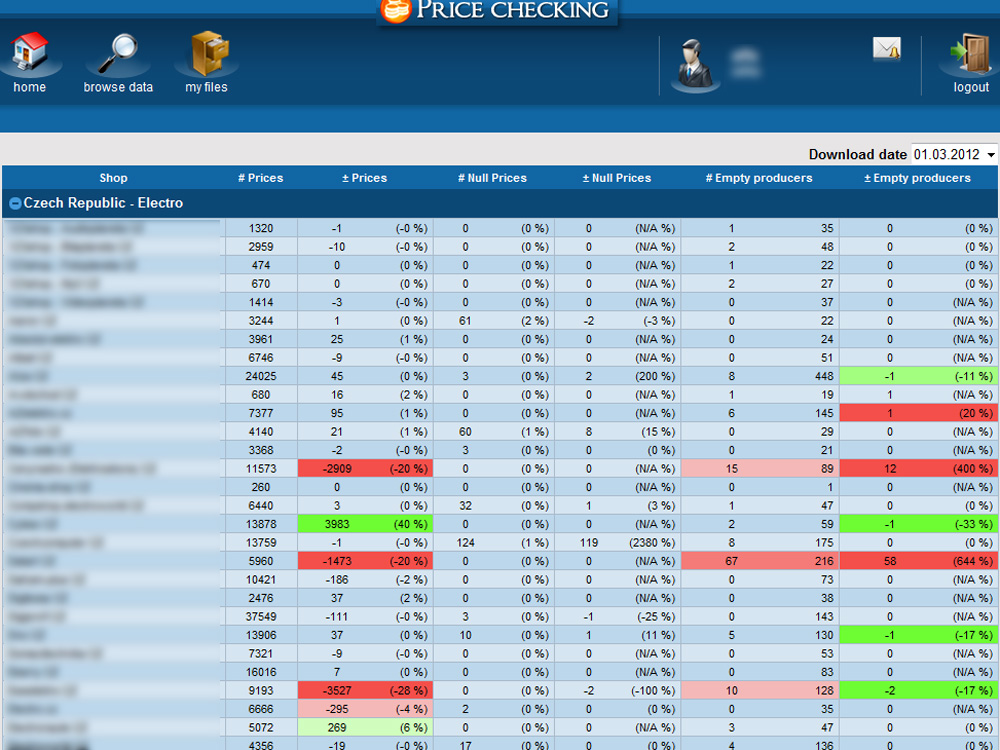
\includegraphics[width=0.9\textwidth]{resources/priceChecking}
	\caption[Price checking]{Ukázka služby Price checking}\label{fig:priceChecking}
\end{figure}

\newpage

\subsection{Pricing intelligence\cite{pricingIntelligence}} 

\textbf{Hlavní funkce}
\begin{itemize}
\item monitorování a srovnávání cen konkurence, vývoj cen a trendů v čase,
\item přehledné výpisy výsledků,
\item u většiny cenových nabídek nutno definovat počet konkurentů,
\item upozornění na změny cen v čase.
\end{itemize}

\textbf{Výstup}
\begin{itemize}
\item formát xsl nebo pdf.
\end{itemize}

\textbf{Prostředí}
\begin{itemize}
\item webové rozhraní.
\end{itemize}

\textbf{Data}
\begin{itemize}
\item nespecifikované data a zaměřený trh.
\end{itemize}

\textbf{Cena}
\begin{itemize}
\item 599 až 4999 Kč měsíčně,
\item minimálně tři měsíce,
\item neomezené sledování produktů a konkurentů je možné pouze s nejvyšším tarifem a po individuální ceně.
\end{itemize}


\subsection{Sledování trhu\cite{sledovaniTrhu}} 
\textbf{Hlavní funkce}
\begin{itemize}
\item sledování cen, pozic, dostupnosti a hodnocení na porovnávačích zboží i jednotlivých obchodech,
\item uchování historie,
\item možné napojení přímo na vlastní internetový obchod,
\item notifikace změn,
\item možnost více účtů s oddělenými přístupy,
\item cenotvorba,
\item detekce cenových spirál (kdo první zlevnil a následující dopady).
\end{itemize}

\textbf{Vstup}
\begin{itemize}
\item xml, xsl nebo manuálně.
\end{itemize}

\textbf{Výstup}
\begin{itemize}
\item xsl nebo webový.
\end{itemize}

\textbf{Prostředí}
\begin{itemize}
\item webové rozhraní.
\end{itemize}

\textbf{Data}
\begin{itemize}
\item srovnávače cen: heureka.cz, zbozi.cz, najnakup.sk, pricemania.sk, ceneo.pl, nokaut.pl, argep.hu, preisroboter.de,
\item přímé sledování na obchodu,
\item z toho plyne záběr na český, slovenský, německý a maďarský trh,
\item aktualizace až několikrát denně.
\end{itemize}

\textbf{Cena}
\begin{itemize}
\item platba za každé vyhledání,
\item individuální cena.
\end{itemize}

\subsection{Pricebot\cite{priceBot}}

Web je datován roku 2015, avšak popis funkcí není dokončený. Obsahuje výplňový text, proto je popis funkcí nekompletní.

\textbf{Hlavní funkce}
\begin{itemize}
\item denní monitoring cen na heureka.cz,
\item možnost sledovat produkty konkurence,
\item poskytuje pravidelný výsledek nalezených cen a vizualizaci změn,
\item notifikace o změnách,
\item notifikace o konkurentech prodávajících za nižší cenu,
\item maximum lze sledovat 600 produktů ,
\item maximum sledovaných konkurentů je 70.
\end{itemize}

\textbf{Vstup}
\begin{itemize}
\item produkty ke sledování.
\end{itemize}

\textbf{Výstup}
\begin{itemize}
\item pdf na email.
\end{itemize}

\textbf{Prostředí}
\begin{itemize}
\item webové rozhraní.
\end{itemize}

\textbf{Data}
\begin{itemize}
\item srovnávač cen Heureka.cz.
\end{itemize}

\textbf{Cena}
\begin{itemize}
\item dle počtů produktů,
\item od 299 do 1299 Kč.
\end{itemize}

\newpage

\subsection{Zahraniční nástroje}
Tyto nástroje jsou obecněji zaměřené a obvykle požadují od uživatele technické znalosti, 
jelikož je nutné přesně specifikovat kde, co a jak je požadováno sledovat. Vzhledem k tomuto omezení není možné
použití přímo provozovateli e-shopů, jelikož těmito znalostmi z povahy práce obvykle nedisponují.
\par
Příklad zahraničních nástrojů:

\begin{enumerate}
\item Screen scraper\cite{ScreenScraper}

  \begin{itemize}
    \item webová služba,
    \item procházení web skrz odkazy,
    \item potvrzování formulářů,
    \item využití interního vyhledávání,
    \item export do širokého množství formátu souborů,
    \item cena: \$549 - \$2,799 za měsíc.
  \end{itemize}
  
\item Web extractor\cite{WebExtractor}

  \begin{itemize}
    \item Windows Aplikace,
    \item procházení zadaných stránek,
    \item hledání stránek pomocí klíčových slov,
    \item export do csv formátu,
    \item cena: \$99 - \$199 jednorázově.
  \end{itemize}


\end{enumerate}

\newpage

\chapter{Analýza týmového projektu}
V této kapitole se budu věnovat řešení vytvořeného v rámci předmětů BI-SP1 a BI-SP2 na ČVUT FIT v akademickém roce 2015/16.
Popíšu cíl, který měl projekt za úkol řešit a jaká měla být výsledná funkcionalita řešení. Dále také vysvětlím základní strukturu
navrženého systému.

\section{Cíl týmového projektu}

V předmětech BI-SP1 a BI-SP2 byl realizován týmový projekt. V souladu s osnovami byl BI-SP1 vytvořen návrh, který
se v BI-SP2 následně implementoval.
\par
Cílem tohoto projektu byla maximální možná míra automatizace získávání informací o produktech prodávaných konkurencí. Důraz byl především kladem na optimalizaci počtu nutných lidských úkonů. Navržený způsob spoléhal v nezbytných krocích na administrátora, u kterého se předpokládala technická zdatnost průměrného uživatele.
\par

\section{Požadovaná funkcionalita}
Požadovaný stav projektu umožňuje uživateli vložit produkty do systému ve formátu \textit{cvs} či \textit{xlsx}, poté pomocí
rozhraní definovat význam jednotlivých sloupců v tomto dokumentu a zvolit požadovanou frekvenci sledování dat.
\par
Systém na základě dat vyhledá obchody, které prodávají vložené produkty. Z nich v definovaných intervalech získává data, ze kterých je vytvořen výstup pro uživatele obsahující především informace o cenách. Výstup lze vizualizovat i na grafech ve webovém rozhraní nebo stáhnout ve formátu
\textit{csv} či \textit{xlsx}.
\par
Proces samotného hledání byl navržen jako soubor více kroků, skládající se z procesů interních částí a interakcí administrátora, který zajišťuje
řešení problémů, které systém nedokáže vyřešit.

\section{Návrh}
Řešení bylo rozděleno na \textbf{část webového rozhraní} a na část zpracovávající interní procesy, nazývanou v této práci 
jako \textbf{interní část}.
Vzhledem k požadavkům na škálovatelnost aplikace se interní část skládá z více samostatných menších služeb - modulů komunikující
spolu pomocí front. Díky tomu, že každý modul zajišťuje určitou funkcionalitu, je možné vytvářet více jejich instancí. Procesy lze 
zpracovávat paralelně a na více serverech, kde je jediné kritérium připojení na systém zajišťující komunikaci.
\par
Uživatelská a interní část spolu sdílejí data pomocí relační databáze\cite{DB}.

\section{Webové rozhraní}

\subsection{Uživatelská část}\label{ch:analysis-front-end}
Uživatelská část obsahuje množinu podstránek určených pro koncové uživatele
služby, klienty.
\par
Uživatelská část umožňuje vytvořit kampaň. Kampaň je proces trvající určitý časový úsek, který sleduje vložené produkty na konkurenčních
obchodech.
V rámci běžící kampaně má poté uživatel možnost vidět vizualizaci získaných dat, případně je umožněn export dat do formátu
\textit{csv} či \textit{xlsx}. Ze zobrazených dat lze zjistit, na kterých webových stránkách je produkt prodáván a za jakou cenu.

\subsection{Část pro administrátory}
Pro přístup do části pro administrátory je nutné, aby měl uživatel speciální práva. Běžný uživatel, tak k této části nemá přístup. Slouží k monitorování kampaní uživatelů a řešení problémů, které systém není schopný 
automaticky vyřešit. Tím je myšleno definování selektorů pro výběr dat z webových stránek, párování produktu ke stránce 
nebo potvrzení zda jsou získaná data validní.

\section{Interní část}
Interní část je rozdělena do samostatných modulů, které spolu komunikují pomocí front. Moduly je možné spustit jako služby ve více 
instancích, kromě modulu Manager. Vzhledem k možnostem front, lze také práci distribuovat na více serverů, aniž by byla ohrožena 
bezpečnost databáze, protože k ní je možný umožnit pouze lokální přístup. Moduly jsou detailněji popsány v následujících podsekcích.
\subsection{Manager}
Manager je hlavní modul, který má jako jediný možnost přímého připojení do databáze. Jeho běžící instance může existovat pouze jednou.
Manager má za úkol plánování práce pro ostatní části systému a samotnou správu komunikace s ostatními moduly. Práce je delegována pomocí
\textit{požadavků}, které jsou odeslány pomocí front jednotlivým modulům. \textit{Odpovědi} a \textit{chyby} reprezentují výsledky.
\subsection{Finder}
Modul Finder získává URL adresy internetových obchodů, které prodávají požadované produkty.
Na nalezeném obchodě poté vyhledává adresy vedoucí na detaily produktů. K tomu je použito interní vyhledávání, které
obchod poskytuje svým zákazníkům. Získané adresy detailů pak obsahují podrobné informace prodávaných produktů.

\subsection{DataProvider}
DataProvider je modul, který zpracovává adresy vedoucí na detaily produktů. Proces modulu reprezentuje následující seznam, kdy každý hlavní bod může skončit uvedenou chybou. Výsledek je odeslán ke zpracování Managerem.
\par
\begin{enumerate}
	\item Stažení stránky.
	\begin{itemize}
	\item Stažení selhalo.
	\end{itemize}
	\item Vyparsování dat pomocí šablony.
	\begin{itemize}
	\item Šablona neexistuje nebo je chybná.
	\end{itemize}
	\item Analýza dat vůči historickým datům (pokud existují).
	\begin{itemize}
	\item Data jsou nevalidní.
	\end{itemize}
\end{enumerate}



\chapter{Vývoj a implementace týmového projektu}
V této kapitole se věnuji průběhu vývoje týmového projektu a vytvořenému řešení. Popíši zvolené postupy při vývoji a 
jaké technologie byly vybrány.
\par
Poslední část rozebírá mou roli v tomto
projektu, protože téma bakalářské práce jsem měl již předběžně vybrané na začátku předmětu BI-SP2.

\section{Vývoj}
Vývoj byl rozdělen do 5 iterací, z nichž každá obsahovala 10 sprintů. 
V každé iteraci bylo definováno jakou musí obsahovat funkcionalitu, která bude na konci iterace prezentována vyučujícímu. Funkcionalita se skládala z jednotlivých úkolů rozložených do sprintů.
\par
Úkoly byly přidělovány jednotlivým členům týmu. Samotné úkoly uchovával systém Redmine\cite{Redmine} a umožňoval sledovat jejich stav.
Úkoly bylo možné v Redmine přiřadit k jednotlivým sprintům a iteracím, což umožňovalo přehled o plnění časového plánu.
\par
Jako verzovací systém byl zvolen systém Git se vzdáleným repozitářem uložený na službě Gitlab\cite{gitlab}. Gitlab poskytuje webové rozhraní pro snadnou správu a možnost spouštění služeb na základě definovaných aktivit v repozitáři. Repozitář se skládal ze 4 částí (větví):

\begin{itemize}
\item Master - hlavní větev uchovávající verze určené k nasazení na produkční server.
\item Develop - vývojová větev obsahující aktuální stav vývoje.
\item Feature - vedlejší větev vytvořená pro konkrétní úkol přidávající novou funkcionalitu.
\item Fix - vedlejší větev určená pro úkoly opravující chybu.
\end{itemize}

Protože práva k modifikaci větví Master a Develop měl pouze vedoucí projektu, musel být pro každou Feature a Fix větev
vytvořen požadavek o zařazení (Merge request). Až po kontrole vedoucím byl požadavek zařazen nebo vrácen k opravě.
\par
Na konci každé iterace byla poslední verze označená pomocí \textit{tagu} a poté prezentována vedoucímu.
Označení bylo zvoleno na základě pořadí iterace. První iterace je označena verzí \uv{0.1}.
\par
Pro vývoj se využil princip průběžné integrace. Každá verze byla zkompilována, otestována a zanalyzována na vzdáleném serveru.
Tyto činnosti zajišťovaly systémy Jenkins\cite{jenkins} a Gitlab. Po změně v repozitáři byl spuštěn úkol v Jenkins. Ten aplikaci sestavil, spustil testy a statickou analýzu kódu 
zajištěnou systémem SonarQube\cite{sonar}. Výsledky publikoval ve svém webovém rozhraní a zároveň v rozhraní Gitlab.  
\section{Implementace}


\subsection{Webové rozhraní}
Webové rozhraní je implementováno v jazyce PHP verze 7. Základem aplikace je aplikační rámec Nette\cite{nette}. Nette
obsahuje nástroje pro automatickou správu závislostí, komunikaci s databází, vytváření bezpečných formulářů, zabezpečení
aplikace, šablonovací systém a rozhraní pro tvorbu testů. 
\par
Nette je navrženo s myšlenkou použití MVC architektury, která odděluje
prezenční a logickou vrstvu. Zkratka MVC značí Model-View-Controller. V případě webového projektu v Nette představují \textit{view} vrstvu šablony, definující vzhled webových stránek. \textit{Controller} vrstva se skládá z presenter tříd obsluhující šablony. \textit{Modelovou} vrstvu  zajišťují třídy servisní, vykonávající logické části aplikace jako 
například práci s \textit{repository} třídami nebo zpracování formulářů. \textit{Repository} se starají o přímou komunikaci s databází.

\begin{figure}[h]\centering
 	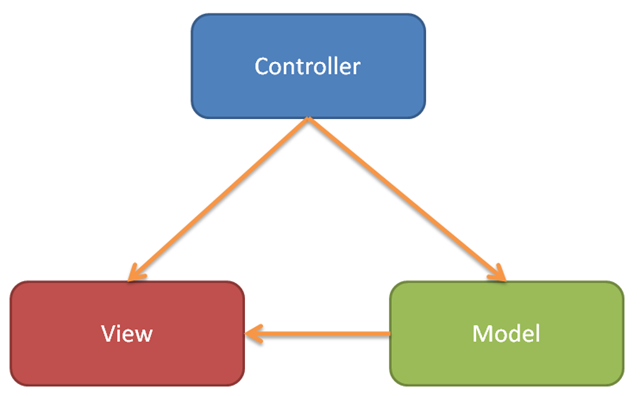
\includegraphics[width=0.7\textwidth]{resources/mvc}
	\caption[MVC]{Vizualizace návrhu MVC (Model-View-Controller)}\label{fig:mvc}
\end{figure}
\par
Snadnou správu závislostí nad externími knihovnami zajišťuje balíčkovací systém Composer\cite{composer}. 
Na základě souboru definující potřebné knihovny a jejich verze jsou staženy pomocí jednoho příkazu z centrálního repozitáře. To zajišťuje jednotné verze
a eliminaci nutnosti knihovny manuálně stahovat či přidávat přímo do repozitáře.
\subsection{Interní část}
Interní část je implementována v jazyce Java verze 8. Sestavení, spouštění testů a správu závislostí zajišťuje Gradle\cite{gradle}.
Umožňuje automatické stažení knihoven. Standardně je nastavený jako zdroj
centrální maven repozitář.\cite{mavenRepo} Maven repozitář uchovává většinu volně přístupných knihoven, v tomto případě všechny, které jsou v rámci tohoto projektu použity.
\par
V rámci sestavení lze pustit testy a další definované úkoly jako například tvorba dokumentace. Projekt používá
doplněk Cobertura\cite{cobertura}, který na základě spuštěné testovací sady vytváří zprávu obsahující pokrytí větví programu.
Díky tomu je možné jednoduše zjistit jaké větve aplikace nejsou otestované.
\par
Aplikace je rozdělena do nezávislých modulů běžící jako služby. Jednotlivé moduly spolu komunikují
pomocí posílání zpráv v definovaných frontách. Komunikaci zajišťuje systém RabbitMQ Server\cite{rabbitMQ} implementovaný v jazyce Erlang. Zprávy jsou serializovatelné objekty, jejichž definice je sdílena napříč všemi moduly.
\par
\textit{Serializace} představuje proces, kdy je objekt serializovaný do posloupnosti bitů, které jsou poslány jako zpráva. 
Vzhledem ke sdílené podobě objektu na obou stranách, lze zprávu jednoznačně deserializovat zpět do původního Java objektu se kterým
je možné dále pracovat.\cite{serialization}
\par
Projekt využívá mnoho volně dostupných knihoven, nejpodstatnější jsou však následující:
\begin{itemize}
\item Google Guice - automatická správa závislostí.\cite{guice}
\item Hibernate - objektově relační zobrazení databázových entit a práce s nimi.\cite{hibernate}
\item Apache Commons - pomocné knihovny pro práci s řetězcemi a soubory.\cite{commons}
\item RabbitMQ - rozhraní pro komunikaci s frontami.\cite{rabbitMQ}
\end{itemize}

\section{Má role}
V druhé části týmového projektu, samotné implementaci, jsem byl vedoucí týmu. Jelikož jsem již měl téma své bakalářské práce vybrané, 
věnoval, jsem se projektu nad rámec předmětu. Kromě povinností vedoucího, které se skládaly z plánování práce a kontroly vytvořené implementace
jsem se věnoval návrhu, který bylo třeba v průběhu semestru pozměnit, jelikož návrh z předmětu BI-SP1 nebyl dostatečný. Jednalo například
o navržení modulu Manager, který byl navržen pouze jako black-box.
\par
Na začátku projektu jsem vytvořil celý ekosystém, tvořený z přidružených služeb použitých při vývoji.
Zde se jedná především o propojení následujících služeb s Gitlabem:

\begin{itemize}
\item Redmine - možnost prokliku na úkol na základě čísla ve zprávě verzované jednotky (commit message).
\item Jenkins - spouštění sestavení aplikace na základě nové verze, oddělené dle jednotlivých větví (hlavní, vývojová, vedlejší) a
				publikace výsledku.
\item SonarQube - zobrazování interaktivního výsledku statické analýzy přímo v rozhraní Gitlab.
\end{itemize}

Samotný SonarQube bylo potřeba nastavit, aby se spouštěl při sestavení aplikace a výsledek se zobrazil v rozhraní
Gitlabu. V rámci sestavení aplikace jsem nastavil spouštění nástroje Cobertura.
Doplňky v Jenkins umožňovaly zobrazení přehledných výsledků, jak je kód pokryt testy viz ukázka \ref{fig:cober-old}. Přesné pokrytí testů mi poté umožňovalo 
jednoduše kontrolovat, jaké části kódu jsou otestované.


\chapter{Zhodnocení týmového projektu}
Pro návaznost na kapitolu o provedených vylepšeních je nejprve nutné uvést v jakém kontextu jsou navrhovány. K tomu je třeba
popsat způsob hodnocení, výsledný stav projektu a jeho funkcionalitu, čemuž se budu věnovat v této kapitole.

\section{Způsob hodnocení}\label{sec:zhodnoceni-typ}
Jako metriky zhodnocení byly zvoleny následující kritéria seřazené od nejpodstatnějšího k nejméně důležitému: 

\begin{itemize}
\item Kritické chyby.
\item Úplnost požadované funkcionality.
\item Rozšiřitelnost.
\item Neefektivní chování.
\item Uživatelská přívětivost.
\item Škálovatelnost.
\end{itemize}

Rozšiřitelnost je hodnocena na základě obecného návrhu, pokrytí testy a počtu chyb statické analýzy kódu. 
Jednotlivým bodům se budu nejprve věnovat v rámci popisu konkrétních problémů. Následně budou shrnuty pomocí tabulky ze které
bude vyvozen závěr analýzy.
\par
Zhodnocení bylo provedeno na základě testování a prozkoumání kódu.
Při testování jsem využil testovací data zobrazené v tabulce \ref{table:testing-data-1}. Postup inicializace systému spočíval ve vytvoření kampaně, namapování produktů a manuálního přidání detailů produktů do databáze.

\begin{table}[h]\centering
    \begin{tabular}{ | l | p{7cm} |}
    \hline
    Produkt & Obchody \\ \hline
    REMINGTON S 8500 &
    	\href{https://www.hair-cosmetics.cz}{hair-cosmetics.cz}\newline
    	\href{https://www.terdom.cz}{terdom.cz}\newline
    	\href{https://www.notino.cz}{notino.cz}\newline
    	\href{https://www.mameradivlasy.cz}{mameradivlasy.cz}\newline
    \\ \hline
    24" Samsung S24D300H & 
    	\href{https://www.alza.cz}{alza.cz} \\ \hline
    \end{tabular}
	\caption{Data použitá k otestování řešení týmového projektu.}
	  \label{table:testing-data-1}
\end{table}

\section{Stav}
Ačkoliv stav projektu odpovídal požadavkům na úspěšné odevzdání, nebyla dosažena implementace všech procesů. 
Tím bohužel nebylo možné reálné použití systému.
\par
Odevzdávaný stav obsahoval funkční webové rozhraní, které se skládalo ze základní funkcionality pro uživatele a administrátory.
Část pro administrátory obsahovala správu uživatelů, evidenci známých obchodů a řešení chyb vzniklých v interní části.
\par
Uživatelská část umožňovala správu a vytvoření kampaní. Splňovala tak návrh z analytické částí \ref{ch:analysis-front-end}.
Na žádost jiného týmu bylo vytvořeno Web API rozhraní, poskytující získané ceny pro daný produktu ve formátu JSON.
\par
Interní část dokázala hledat nové data na již uložených adresách detailů. Manager vybral adresy detailů pro zpracování, vytvořil
jednotlivé požadavky obsahující potřebná data a odeslal je k zpracování do DataProvideru. DataProvider obsah adresy stáhnul, vyparsoval a výsledek zanalyzoval vůči historickým datům. Analýza se skládala z kontrol velkých výkyvů cen a rozdílných identifikátorů produktu. Pokud všechny části proběhly bezchybně, byly data odeslány pro zpracování Managerem.
\par
Systém se korektně zachoval i pokud při stažení, parsování nebo analyzování byla objevena chyba. Proces zastavil, výsledek označil jako chybný
a odeslal chybnou odpověď. Zpracování Managerem zajistilo, že bylo možné chybu vyřešit administrátorem ve webovém rozhraní. Po vyřešení chyby systém zareagoval a vytvořil opětovný požadavek.

\begin{figure}[h]\centering
 	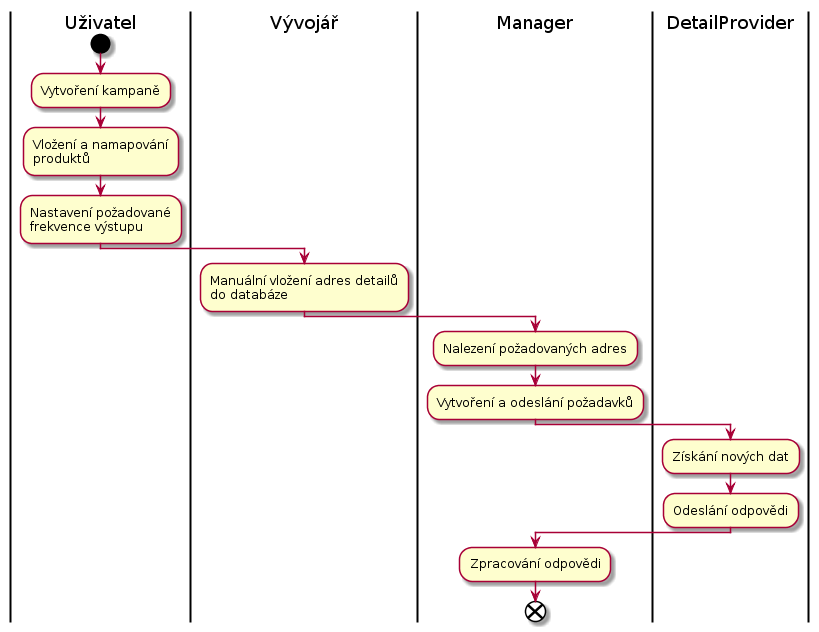
\includegraphics[width=1.0\textwidth]{resources/legacy-process-activity}
	\caption[Diagram zobrazující vytvoření kampaně a nalezení nových dat v původním řešení týmového projektu]
	{Diagram zobrazující vytvoření kampaně a nalezení nových dat v řešení týmového projektu.}\label{fig:legacyprocess-activity}
\end{figure}

\section{Nedostatky}

\subsection{Vytváření požadavků pro ProductProvider}
Některé nedostatky byly úzce spjaty s tím, jak aplikace plánovala práci. Plánováním práce je myšlen proces
nalezení adres detailů produktů pro které je požadováno získat aktualizované data. Z adres jsou vytvořeny a odeslány požadavky pro ProductProvider.
\par
Prvotním kritériem hledání jsou adresy detailů. Ty se mohou vyskytovat v různých stavech. Systém je vybral v 
následujícím pořadí:

\begin{itemize}
\item Adresy, které mají produkty v zaplacené kampani.
\item Adresy bez produktů.
\item Adresy, pro které neexistuje šablona pro parsování.
\item Adresy, které mají vyřešenou chybu.
\end{itemize}

Z této množiny bylo vybráno prvních 10 adres, odebrány již odeslané a takové které mají nevyřešenou chybu. Opakované spuštění v předdefinovaném 
intervalu zajistilo vytvoření požadavků pro všechny požadované adresy.
\par
Další nedostatek se skládal z ukládání stavu do databáze. Část nejdůležitějších atributů vytvářeného požadavku byla uložena do databáze 
s příznakem odesláno. Tento příznak bylo nutné uchovávat i u chyb šablon nebo analyzátoru, kde je potřeba označit zpracování Managerem. 
\par
Při neúspěchu odeslání požadavku už příznak u chyb nebyl změněn. To způsobilo, že chyba zůstala navždy s příznakem \uv{zpracována}, ačkoliv
se příslušný požadavek nepodařilo odeslat.

\subsection{Neefektivní chování modulu Manager a ProductProvider}\label{ch:manager-pd}
V rámci testování jsem zjistil, že v případě chyby při parsování stránky není použit uložený HTML dokument. I když dokument do databáze
při zpracování chyby ukládán byl.  
\par
Manager vyhledal korektně adresy detailů, ale vytvoření objektu představující požadavek bylo pro všechny adresy stejné. 
Ztracení důvodu z jakého byla adres původně vybrána, způsobilo nemožnost jednoduchého uložení HTML dokumentu do požadavku. Každý požadavek znamenal opětovné stažení příslušné stránky.

\subsection{Chyby analyzování}
Poslední fáze procesu v modulu ProductProvider byla navržena jako analyzování získaných dat vůči již dříve uloženým. Implementace analyzátoru 
spouštěla jednotlivé validace, jejíchž logika se nacházela v oddělených třídách. 
Analýza kontrolovala zda se shoduje získaný EAN, název a modelové číslo, vůči uloženým identifikátorům. Pokud na jedné ze stran hodnota neexistovala, byly data označená, že jsou pravděpodobně chybná. 
\par
Dále probíhala kontrola získané ceny \uv{s} a \uv{bez} DPH oproti dříve získaným cenám na stejné adrese. Kontrola porovnala průměr historických hodnot s hodnotami získaných cen. V případě, že rozdíl byl větší jak 25\%, byl výsledek označen jako chybný.
\par
Po odeslání a přijetí chyby, Manager ji uložil do databáze pro administrátora k vyřešení. Administrátor pak mohl 
označit, zda je to opravdu chyba nebo se toto hlášení má do budoucna ignorovat.
\par
\subsubsection{Problémová implementace}
Pokud validační třída objevila nežádoucí data, vyhodila výjimku obsahující informace o chybě. Tento způsob řízení programu však způsoboval, že celá validace skončila při první chybě. Zároveň výjimka obsahovala pouze typ validace. 
Skončení po první validaci způsobovalo, že administrátor musel řešit chyby postupně. 
Pokud stránka obsahovala více chyb, byl po každém vyřešení vytvořen nový požadavek, který způsobil další chybu.
\par
Samotné administrátorské rozhraní obsahovalo pouze informaci o typu chyby. Příčina byla nedostatečná práce s existující daty ve webovém rozhraní
a zároveň nebyly ukládány detailnější informace o chybě. 

\subsection{Vytváření chyb šablon}
Jako nedostatek se ukázalo plánování práce založené na kritériu, kdy jsou k vytvoření požadavku vybrány všechny adresy, které neobsahují šablonu.
Myšlenka byla taková, že pro vytvoření samotné šablony, je nutné nejdříve stránku stáhnout, nechat vytvořit chybu parsování
a následně ji vyřešit.
\par
Systém však odeslal požadavek pro všechny uložené adresy na obchodě. Každá znamenala chybu šablony, které musel administrátor postupně vyřešit.

\subsection{Modul Finder}
Modul Finder nebyl zapojený do systému. Existovala pouze hlavní implementace interních procesů Finderu, jejíchž funkčnost byla
pouze ověřena jednotkovými testy. Neexistující rozhraní pro práci s frontami a chybějící příslušné třídy Managera, které zajišťují vytváření příslušných požadavků neumožňovaly ověření celkové funkcionality této části. Z tohoto důvodu nebyl systém jako celek vhodný pro jakékoliv reálné použití, jelikož
jediná možnost jak využít funkcionalitu interní částí, bylo vytvořit SQL insert skripty, obsahující adresy detailů produktů
a ty spustit nad databází, kterou systém používal.
\par
Další důsledek byla neexistence procesu párování produktů. Finder byl navržený tak, že po nalezení internetového obchodu
pomocí interního vyhledávání nalezne detaily produktů, u kterých je velká pravděpodobnost, že patří hledanému produktu.
Zda se jedná o správné adresy je třeba ověřit. Výsledkem hledání mohou být adresy, které nepatří hledanému produktu. Po získání hodnot ze stránky se musí nežádoucí adresy vyloučit a ostatní spárovat s uloženými produkty.
\subsection{Plánování práce}
Projekt neobsahoval plánování práce vůči požadovanému intervalu, kdy mají být nová data
staženy. Aktuální stav hledal pouze adresy produktů, které se nachází v zaplacené kampani nebo měly vyřešenou chybu.
\subsection{Škálovatelnost}
Původní návrh počítal se škálovatelností aplikace na více serverech, kde je možné vytvořit neomezený počet instancí DataProvider a Finder. Reálný stav na konci projektu však tuto možnost neumožňoval. Interní část běžela jako jedna služba rozdělená do více modulů. 
Instance všech modulů probíhala v Managerovi, který musel mít přímou závislost na ostatních modulech.
\subsection{Obecný návrh a testy}\label{ch:architecture-tests}
Implementace samotná byla velmi nepřehledná. Vykytovaly se prvky značící špatný návrh aplikace.
Zde bych rád zmínil například dlouhé a nepřehledné metody v
DataProviderServiceImpl a AbstractFinderUrlListWorkerImpl, kde přestože jejich velikost 
nepřesahovala 60 řádků bylo velmi obtížné zjistit, co mají vykonávat. Problém byly také velké třídy
jako například DataProviderServiceImpl zajišťující celý proces v modulu DataProvider.
\par
Je nutné podotknout, že spousty špatných konstrukcí bylo eliminováno již v průběhu vývoje týmového projektu.
První důvod byla statická analýza kódu detekující konstrukce, které jsou zdrojem častých chyb. Statická analýza
však nebyla schopná najít všechny problémy. Druhý důvod byla moje kontrola při schvalování vytvořeného kódu pro 
zadaný úkol. Z důvodu časové tísně nebyl vždy prostor na to vrátit kód k přepsaní a opravení všech nedostatků. To způsobilo, že
se vědomě dostaly do hlavních větví konstrukce, které nebyly považovány za ideální. Myšlenkou bylo, že budou přepracovány později, což se ne vždy povedlo.
\par
Další problém návrhu byly procesy v DataProvider modulu řízené pomocí výjimek obsahující 
přídavné informace. A to i v případech, kdy byl takový výsledek očekávaný nebo dokonce chtěný. 
Toto použití je však v rozporu ideou použití výjimek, které mají signalizovat \textit{neočekávaný} stav, kdy není možné dále pokračovat.\cite{exception}
Pro uchování přídavných informací bylo nutné vytvářet výjimky vlastní, které obsahují údaje o chybě.
\par
V kritických částech chyběly některé důležité testy, jelikož třídy snažící se dělat více věcí najednou, by bylo velmi
složité otestovat. Chybějící testy se vykytovaly například u následujících částí: databázová vrstva, fasády, vytváření požadavků pro DataProvider,
hlavní servisní třída DataProvideru nebo validace dat analyzátorem. Z tohoto důvodu jakákoliv oprava nebo implementace nových požadavků 
mohla narušit stávající funkcionalitu bez možnosti rychlého ověření. Tím by mohla být jakákoliv změna velmi časově náročná, s velmi nejistým konečným výsledkem.

\begin{figure}[h]\centering
 	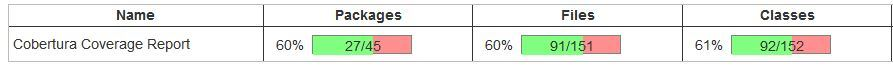
\includegraphics[width=1.0\textwidth]{resources/cobertura-report-old-1}
 	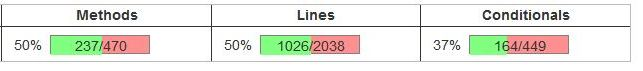
\includegraphics[width=0.7\textwidth]{resources/cobertura-report-old-2}
	\caption[Pokrytí testy vytvořeného řešení]{Pokrytí testy vytvořeného řešení. Získáno pomocí nástroje Cobertura. Vizualizace
	výsledků byla vytvořena při sestavení na Jenkins s příslušným doplňkem.}\label{fig:cober-old}
\end{figure}

\section{Shrnutí}\label{ch:project-analysis}

Na základě shrnutí nedostatků v tabulkách \ref{table:analysis-old1} a \ref{table:analysis-old2} je možné prohlásit, že pro základní použití systému by byla nutná oprava všech kritických chyb a doplnění o chybějící funkcionalitu. Pro zajištění jednoduchého zapracování změn bude také nutný refaktoring, úprava návrhu a doplnění základních testů, které chybějí.
Výsledek statická analýzy kódu ukázal, že počet nalezených chyb je minimální, což bylo způsobeno jejím průběžným použitím při vývoji. Při přezkoumání byly i přes výsledek analýzy kódu nalezeny nežádoucí konstrukce.
\par
Problémy týkající se nedostatečné přívětivosti administrátorského rozhraní způsobují nepohodlné použití systému a bylo by vhodné je též zapracovat.
\par
V případě provedení výše uvedených změn, předpokládám
snadnou možnost oprav částí týkající se neefektivního chování.
Neefektivita se může negativně odrazit při velké zátěži a proto by měla být odstraněna.
Škálovatelnost má vzhledem k ostatním problémům nejnižší prioritu. Z tohoto důvodu není nutné se škálovatelnosti věnovat.

\begin{table}[h]\centering
    \begin{tabular}{ | l | p{7cm} |}
    \hline
    Typ & Popis \\ \hline
    Kritické chyby &
    	\begin{itemize}
  			\item V případě chybného odeslání není chyba šablony nebo analyzátoru znova zpracována.
  		\end{itemize}\\ \hline
	\hline
    Úplnost funkcionality & 
    	\begin{itemize}
  			\item Systém nevyhledává internetové obchody.
  			\item Systém nevyhledává adresy detailů produktů.
  			\item Systém neplánuje práci v požadovaných intervalech.
  			\item Neexistence procesu párování.
  		\end{itemize} \\ \hline
	\hline
	Rozšiřitelnost  & 
		\begin{itemize}
  			\item Návrh tříd byl vyhodnocen jako nevhodný pro rozšiřování.
  			\item 60 \% pokrytí testy dle nástroje Cobertura.
  			\item 3 kritické chyby statické analýzy kódu.
  			\item 1 minoritní chyba statické analýzy kódu.
  		\end{itemize} \\ \hline
    \end{tabular}
	\caption{První část přehledu nedostatků vytvořeného týmového řešení.}
	  \label{table:analysis-old1}
\end{table}
\begin{table}[h]\centering
    \begin{tabular}{ | l | p{7cm} |}  
    \hline
    Typ & Popis \\ \hline
	Neefektivní chování & 
		\begin{itemize}
  			\item Stránka je nově stažena  v každémpožadavku (i v případě uložení při chybě).
  			\item Každá chyba analyzátoru znamená samostatný požadavek a chybu.
  			\item V případě neexistenci šablony detailu pro obchod jsou vytvořeny požadavky pro všechny adres, kdy každá způsobí chybu parsování, kterou je nutné vyřešit.
  		\end{itemize} \\ \hline	
	\hline
	Uživatelská přívětivost & 
		\begin{itemize}
  			\item Nutnost řešit chyby analyzátoru po jedné.
  			\item Řešené chyby neobsahují bližší informace (informace o chybě, vyparsované hodnoty, použitá adresa detailu).
  		\end{itemize} \\ \hline	
	\hline
	Škálovatelnost & 
		\begin{itemize}
  			\item Nemožnost vytvořit více instancí modulů.
  		\end{itemize} \\ \hline
    \end{tabular}
	\caption{Druhá část přehledu nedostatků vytvořeného týmového řešení.}
	\label{table:analysis-old2}
\end{table}


\chapter{Návrhy na vylepšení}
V této kapitole se věnuji návrhům na možná vylepšení. Samotné implementaci se poté věnuji v následující kapitole. 
Nedostatky, které byly zjištěny až v průběhu implementace vylepšení a nebyly zároveň i opraveny, budou zmíněny v kapitole týkající se zhodnocení
provedených vylepšení. Při implementaci jsem funkčnost provedených změn průběžně ověřoval pomocí jednotkových testů a testovacích dat použitých při zhodnocení týmového projektu. Hledání produktů a párování bylo ověřováno na základě dat nových. Těmto datům se budu podrobněji věnovat v další kapitole, \textit{Zhodnocení provedených vylepšení}.
\par

\section{Refaktorování stávajícího řešení}
Na základě přezkoumání kódu bylo určeno, že by bylo vhodné provést refaktorování, jelikož existujícím kódu není možné stavět opravy nebo přidání nových funkcionalit. Příčinou jsou konstrukce jako zneužívání výjimek, dlouhé metody, velké třídy nebo dlouhé seznamy parametrů.
Z těchto důvodů je třeba vhodně interní část refaktorovat tak, aby bylo možné kód lépe udržovat a rozvíjet. Provedené změny důkladně 
otestovat pomocí jednotkových testů.
\par
V rámci refaktorování je nutné se pokusit zachovat co nejvíce původního kódu, obzvlášť takového, kde je ověřena funkcionalita.
Dále pro větší přehlednost přesunout všechny servisní třídy do samostatného balíku a sjednotit je.
\par
Při úpravách týkající se rozdělování jednotlivých tříd do samostatných jednotek, musí být dán důraz na jejich přehledné a rozšiřitelné komunikační rozhraní.

\subsection{Řízení aplikace}
Chování modulu ProductProvider je řízeno pomocí chytání výjimek obsahující informace o chybě. 
Výjimky by bylo vhodné odstranit a návratové hodnoty změnit na objekt obalující celkový výsledek. Tento návrh ulehčí implementaci procesů, kde není žádoucí
skončit při první chybě. Kód bude možné lépe rozdělit a metody následně zkrátit, což výrazně zlepší přehlednost kódu.

\section{Plánování práce}
Samotná logika plánování práce, nebo-li nalezení adres detailů produktů, které chceme použít při vytváření požadavků, se ukázala být nedostatečná. Chybí požadovaná funkcionalita, tedy použití intervalu určující, kdy je požadován nový výstup.
\par
Nový návrh by měl hledat adresy podle těchto kritérií:

\begin{itemize}
\item Adresy, které mají produkty v aktivní kampani a požadovaný interval hledání odpovídá aktuálnímu dni.
\item Adresy bez produktů.
\item Adresy, pro které neexistuje šablona pro parsování.
\item Adresy, které mají vyřešenou chybu.
\end{itemize}

Po nalezení těchto disjunktních množin a odstranění duplicit, vyřadit adresy, které z nějakého důvodu nevyhovují svým stavem.
Nežádoucí stavy jsou tyto:

\begin{itemize}
\item Pro obchod existuje nevyřešená chyba šablony.
\item Existuje nevyřešená chyba analyzátoru.
\item Požadavek pro adresu byl již odeslán.
\end{itemize}

Z důvodu možnosti, že nežádoucí stavy bude pravděpodobně požadované přidat či odebrat, je potřeba implementaci navrhnout tak, aby bylo možné kontroly kdykoliv modifikovat bez velkých zásahů do interní funkcionality.

\section{Oprava komunikace Manager - ProductProvider}
Vzhledem k problémům popsaných v kapitole \ref{ch:manager-pd} je požadováno komunikaci modulů Manager a ProductProvider optimalizovat.
Neefektivní chování by se mohlo ukázat jako velký problém při zpracování velkého počtu dat z důvodu nutnosti opakovaného
stahování webových stránek. 
\par
Při analýze kódu se ukázalo, že v aktuálním návrhu aplikace není možné tuto funkcionalitu jednoduše implementovat, aniž by se nejednalo o rychlou opravu neefektivním řešením. Oprava by znamenala, že pro každou vytvářenou adresu se systém musí pokusit najít
existující chybu. Hledání by tak probíhalo ve většině případů zbytečně, jelikož chyba by neexistovala.
\par
Korektní oprava je úzce spjata s předchozími kapitolami. Především s refaktorováním a úpravou plánování práce. 
Pokud úprava plánování zachová informaci o důvodu udávající, proč je adresa pro vytvoření požadavku zařazena, stačí chybu obsahující staženou stránku nalézt pouze u příslušných požadavků.
\par
Informace důvodu nalezení by však měla být zachována i při odesílání. V rámci odesílání požadavků jsou nastavovány příznaky o odeslání a zpracování chyby. Když se požadavek nepodaří odeslat musí existovat možnost příznak změnit.
\par
Z hlediska použití stránky v DataProvideru stačí zkontrolovat, zda požadavek stránku uchovává a v kladném případě ji použít pro
parsování.

\section{Spojení chyb analyzátoru a vylepšení rozhraní} \label{analyser-join}
Analyzátor provádí kontrolu získaných dat. V případě podezření o nevalidních datech je vytvořena chyba určená k vyřešení
administrátorem. Validace kontrolují ekvivalenci identifikátorů vůči již uloženým a velké výkyvy cen na daném obchodu.
\par
Administrátor má možnost chybu vyřešit a uložit příznak, aby se chyba do budoucna ignorovala. 
Jediné informace, které má při řešení k dispozici je typ validace.
Webové rozhraní ani nemá možnost zobrazit dodatečné informace o chybě, protože nejsou ukládána. Proto by interní část měla takové informace
zpracovat a uložit.
\par
V případě adresy, která obsahuje více chyb, je nutné řešit každou samostatně. Po každém vyřešení se musí počkat na zpracování interní částí.
Pro vylepšení administrátorské rozhraní je požadováno chyby spojit do jedné, tak aby bylo možné vyřešit všechny chyby analyzátoru najednou.

\section{Monitorování}
Na virtuálním serveru probíhá sestavení aplikace, včetně všech dodatečných procesů. Zároveň zde běží vývojová a produkční verze interní i webové části.
Momentální stav poskytuje pouze omezenou možnost, jak sledovat využití prostředků virtuálního serveru.
\par
Pro lepší přehled běžících prostředků by bylo vhodné zvolit monitorovací službu umožňující sledování
probíhajících procesů na serveru, včetně vytížení a stav zobrazuje na externí službě, která bude funkční i v případě, kdy server neběží.

\section{Získání adres obchodů a příslušných detailů produktů}
Interní část vyžaduje ke své funkcionalitě již uložené adresy detailů produktů. Pomocí nich jsou získávána nová data o produktech.
Původní návrh počítal s modulem Finder, který se nepodařilo zapojit v rámci týmového projektu. Ten 
měl za úkol hledat internetové obchody na cenových srovnávačích a na nich pomocí vyhledávaní nalézt konkrétní adresy.
\par
Funkce Finderu je navržena jako duální, zajišťuje jak hledání samotných obchodů, tak i detailů adres. Komunikační třída představující příslušný požadavek, proto musí obsahovat příznak o jaký typ požadavku se jedná. Jelikož předávané informace
jsou odlišné, vytvořený požadavek obsahuje velké množství prázdných hodnot, což přispívá k celkové nepřehlednosti.
\par
Z tohoto důvodu navrhuji rozdělení Finderu na dva samostatné moduly. První bude zastávat funkci hledání obchodů a druhý
vyhledávat na obchodu a získávat požadované adresy detailů produktů na daném obchodě.
\par
Samotné hledání obchodů pak není kritická funkcionalita a je možné ji nahradit manuálním vložení internetových obchodů pomocí webového rozhraní.


\section{Párování produktu}
Po nalezení adresy detailu produktu, jejím stažení v DataProvider modulu a následném vyparsování hodnot je třeba adresu spárovat s 
produktem uloženým v databázi. Příčinou nutnosti párování je, že po nalezení adresy detailu není jisté, jestli opravdu patří produktu, pro který 
byla nalezena. 
\par
Párování musí být provedeno s velkou jistotou. Z tohoto důvodu navrhuji vytvořit proces, který se nejprve pokusí produkt spárovat na základě shody některého z identifikátoru, což představuje název, modelové číslo nebo EAN produktu. 
\par
Proces není možné zcela zautomatizovat, jelikož část internetových obchodů nemusí poskytovat informace totožné s těmi uloženými.
Obchod může používat odlišný název. Odlišnosti identifikátorů může způsobit například jiná barva nebo přidaná velikost za nebo před modelové
číslo. Jako řešení se jeví hledat podřetězec modelového čísla a EANu, což řeší problém pokud je ze stránky vyparsován text okolo
identifikátoru. Obchod také může poskytovat pouze název. To lze demonstrovat na obchodu \textit{glamot.cz}, například
pro produkt 
\href{https://www.glamot.cz/p/19128/difuzer-k-vysouseci-babyliss-pro-difuser-murano}{BaByliss PRO Difuser Murano \textit{[cit. 24.4.2017]}}.
\par
V případě neúspěchu párování, musí existovat možnost produkt spárovat manuálně, akcí administrátora. 
Výše uvedený proces spoléhá na to, že vložená data jsou při vytváření kampaně validní. V případě nevalidních dat jako
příliš obecných a krátkých názvů by párování mohlo proběhnout chybně.


\section{Neimplementované návrhy}
\subsection{Pokročilé párování produktu}
Párování produktu lze vylepšit o možnost uchování více hodnot u identifikátorů produktů. V praxi by to znamenalo, že produkt je vytvořen 
s hlavními identifikátory. V průběhu hledání na obchodech a po potvrzení administrátorem by bylo možné uložit identifikátory alternativní.
\par
Alternativní název by bylo možné využít při párování produktu, pokud by při použití hlavního názvu nebyla nalezena shoda.

\subsection{Uchování a využití hodnot z nespárovaných adres}
Vyhledáváním na obchodu je zpravidla výsledek, který obsahuje více adres detailů produktu. Na všech získaných adresách je proveden pokus o spárování, takže jsou nejdříve vyparsována příslušná data z těchto stránek. Pokud systém neuchovává všechny existující produkty prodávané na internetu, pak část adres vždy
náleží neznámým produktům a není v době hledání potřebná. Získáná data by bylo možné uchovávat a pokusit se je spárovat při přidání nových produktů do databáze.
To umožní odlehčení zátěže na stahování stránek a urychlí celý proces nalezení detailu adresy a párování produktu.


\chapter{Realizace vylepšení}\label{ch:realisation}
Kapitola Realizace vylepšení se věnuje implementovaným vylepšením. Popisuje, jak byly navržené změny provedeny.
V průběhu realizace byly objeveny nové nedostatky, z nichž některé byly také zpracovány, i když se s nimi původně nepočítalo.
Změny jsou v repozitáři webového rozhraní a interní části přehledně označeny. Původní verze týmového projektu byla označena jako
tag \textit{v0.53}, realizované vylepšení jsou označeny jako \textit{v0.6}.

\section{Refaktorování stávajícího řešení}
První krok realizace bylo refaktorování stávajícího řešení. Zde bylo provedeno především přesunutí tříd do jednotného balíčku, 
rozdělení tříd, odstranění přebytečných výjimek, zkrácení a zmenšení počtu parametrů metod.

\subsection{Servisní třídy}
Pro větší přehlednost byly všechny servisní třídy přesunuty do nadřazeném balíčku \textit{service}. 
Servisní třídy jsou takové, které nespadají do ani jedné z těchto skupin:

\begin{itemize}
\item Obsluha frekvenčního probouzení aplikace v daném intervalu.
\item Rozhraní komunikující s frontami.
\item Třídy přistupující k databázi (DAO).
\item Fasády, které obalují komunikaci servisních a DAO tříd.
\item Konfigurační soubory automatické správy závislostí.
\item Komunikační třídy.
\item Pomocné třídy.
\end{itemize}

Třídy jsem pojmenoval pomocí nové konvence, kdy důležité servisní třídy obsahují prefix zkratky modulu, kterého se týkají
a postfix \textit{Service}. Důvodem byla větší přehlednost v projektu, kdy docházelo k podobným názvům napříč moduly.
\par
Změnu lze demonstrovat například na třídě zajišťující získávání dat ze stažené stránky. Třída \textit{cvut.fit.dataprovider.parser.ParserImpl} byla pak změněna na \textit{cvut.fit.dataprovider.service.parser.DPParserServiceImpl}.\footnote{Uvedené názvy jsou včetně 
nadřazených balíčků. Název třídy je v prvním případě pouze \textit{ParserImpl}.}

\subsection{Řízení aplikace}
Aplikace, především v DataProvider modulu byla řízena pomocí výjimek, které způsobovaly problémy v návrhu a samotné funkcionalitě.
V návaznosti na návrh byly nahrazeny úpravou návratového typu, který obsahuje příznak výsledku 
a doplňující informace.
\par
Návratový typ lze demonstrovat na následují třídě \textit{DPParserRespose}\footnote{Ukázka třídy je zkrácena oproti reálné verzi.}, která je vrácena v DataProvider modulu po provedení parsování.

\begin{lstlisting}[language=Java]
/**
 * Entity to keep parsed response. Almost every 
 * attribute can be null, 
 * so getters return {@link Optional} of nullable type.
 *
 * @author Jakub Tucek
 * @created 24.1.2017
 */
public class DPParserResponse {

    /**
     * Flag for keeping result of parsing
     */
    boolean finishedProperly;

    /**
     * Parsed name of the product
     */
    private String name;

    public boolean isFinishedProperly() {
        return finishedProperly;
    }

    public void setFinishedProperly(
    	boolean finishedProperly) {
    	
        this.finishedProperly = finishedProperly;
    }

    public Optional<String> getName() {
        return Optional.ofNullable(name);
    }

    public void setName(String name) {
        this.name = name;
    }
}
\end{lstlisting}

Třídy zajišťující parsování parsování hodnot ze stažené stránky v modulu DataProvider používají uvedenou strukturu.
Ukázka kódu ukazuje použití příznaku označující, zda parsování proběhlo úspěšně. Další důležitý prvek
je zapouzdření proměnných uchovávající data\cite{encapsulation}, jelikož přístup k proměnným je umožněn pouze pomocí \textit{get} a \textit{set} metod.
\par
Metody \textit{get} jsou oproti standardnímu návrhu pozměněny a nevrací přímo proměnnou, ale \textit{Optional} této proměnné.
Optional je kontejner, který může obsahovat požadovanou hodnotu\cite{optional} nebo být prázdný. 
Před přístupem k hodnotě nepřímo vyžaduje ověření stavu objektu. Očividnost prázdnoty návratové hodnoty nutí vývojáře s touto možností počítat, což
omezuje výskyt nežádoucích výjimek, především \textit{NullPointerException}\cite{nullPointerException}.
\par
Po nahrazení návratovými typy, jsou výjimky použity pouze v případech, kdy nastal neočekávaný stav a je nutné přerušit následující akce.

\subsection{Odstranění výjimky a spouštění validací}
Odstranění výjimek z interní části lze demonstrovat na třídách zajišťující analyzování získaných výsledků v modulu DataProvider. Hlavní změny v této části jsou tři.
\par
První je přesunutí hlavního rozhraní \textit{Analyser} a jeho implementace
\textit{AnalyserImpl} z balíčku \textit{cvut.fit.dataprovider.analyser} 
do  \\
\textit{cvut.fit.dataprovider.service.analyser}. 
\par
Druhá změna představuje změnu rozhraní, kdy bylo potřeba
zmenšit počet parametrů a odstranit výjimku, která byla vyhozena v případě nalezení chyby. 
\par
Třetí změnou je samotné spouštění validací. V původním řešení byla třída závislá na všech příslušných validacích, které spouštěla.
Skončila však vždy při první chybě, což je jedna 
z příčin chování, na kterou reaguji v návrhu na spojení chyb analyzátoru, \ref{analyser-join}.
\par
Vytvořil jsem nový návrh, který je v modifikovaných verzí použit i na ostatních místech interní části. Analyzující servisní třídě jsem odebral jednotlivé závislosti na konkrétních validacích a nahradil kolekcí obsahující validační rozhraní. Jednotlivé implementace validačního rozhraní jsou pak do třídy nastaveny konfigurační třídou automatické správy závislostí.
\par
Validačnímu rozhraní byl změněn návratový typ na \textit{Optional} třídy obsahující zprávu o chybě. Pokud chyba nenastala, vrací
prázdnou hodnotu. Implementace validačního rozhraní byly rozděleny podle toho, jakou hodnotu kontrolují.
Při úpravě validací jsem zjistil, že základní validace lze rozdělit na dvě skupiny: validace řetězce a čísla.
\par
V případě těchto skupin se vytvořený kód lišil pouze v tom, jaká hodnota se má získat ze získaných dat a z dat již uložených.
Poslední rozdíl byl pouze v chybové hlášce. Z toho důvodu jsem společnou logiku obou skupin implementoval
pomocí abstraktní a generické třídy \textit{AbstractAnalysis}. Vlastnosti kontrol jednotlivých skupin zajišťují třídy \textit{AbstractStringAnalysis} 
nebo \textit{AbstractPriceAnalysis}. Výsledná validace kontrolující získaný název s uloženým vypadá následovně:

\begin{lstlisting}[language=Java, caption={Validace kontrolující hodnotu získaného jména produktu.}]
/**
 * NameAnalysis is extension of {@link AbstractStringAnalysis} for analysing Name.
 *
 * @author Jakub Tucek
 * @created 27.1.2017
 */
public class NameAnalysis extends AbstractStringAnalysis {

    /**
     * {@inheritDoc}
     */
    @Override
    boolean skipAnalysis(DataProviderRequest request) {
        Optional<ComAnalyserFlags> analyserFlags = request.getAnalyserFlags();
        return analyserFlags.map(ComAnalyserFlags::isIgnoreDifferentName)
                .orElse(false);
    }

    /**
     * {@inheritDoc}
     */
    @Override
    Optional<String> getOptionalProperty(DPParserResponse parserResponse) {
        return parserResponse.getName();
    }

    /**
     * {@inheritDoc}
     */
    @Override
    List<String> getComProductValues(ComProduct comProduct) {
        return comProduct.getNames();
    }

    /**
     * {@inheritDoc}
     */
    @Override
    AnalysisErrorMessage generateAnalysisErrorMessage(String comProductValue, String parsedValue) {
        return new AnalysisErrorMessage()
                .withErrorMessage(
                        String.format("Parsed name value[%s] doesn't match known name value[%s]",
                                parsedValue, comProductValue)
                )
                .withErrorType(AnalysisErrorType.DIFFERENT_NAME);
    }
}
\end{lstlisting}
Jednotlivé validace implementují pouze metody vracející příslušná data se kterými validace pracuje. Jedná se o vyparsované hodnoty, historická
data a příznak určující, jestli administrátor nastavil ignorování chyby.
Poslední implementovaná metoda vytváří informace o případné chybě. Tuto informaci je poté
možné využít pro detailnější zobrazení v administračním rozhraní. Vylepšení samotného webového rozhraní chyb analyzátoru se věnuji v následující sekci.
\par
Konečné spuštění validací bylo ve výsledku zkráceno na metodu obsahující jeden řádek kódu, ačkoliv tento řádek
obsahuje více zřetězených volání.
\par
\begin{lstlisting}[language=Java, caption={Upravená implementace hlavní metody ve třídě zajišťující spouštění validací analyzátoru.}]
    /**
     * Runs analysis for given {@link DataProviderRequest} and {@link DPParserResponse}.
     * Error are returned as list of {@link AnalysisErrorMessage}.
     * Injected set of {@link Analysis} is executed one by one, result unwrapped and kept if present.
     * Set of analysis result error messages is returned.
     *
     * @param request        dp request
     * @param parserResponse parsed data
     * @return list of errors or empty (if result was valid)
     */
    @Override
    public List<AnalysisErrorMessage> runAnalysis(DataProviderRequest request, DPParserResponse parserResponse) {
        return analysisSet.stream()
                .map(x -> x.analyse(request, parserResponse))
                .filter(Optional::isPresent)
                .map(Optional::get)
                .collect(Collectors.toList());

    }
\end{lstlisting}

\begin{lstlisting}[language=Java, caption={Původní implementace hlavní metody ve třídě zajišťující spouštění validací analyzátoru.}]
    /**
     * Analyses the new product info in comparison with the history
     *
     * @param newInfo        the new product info to be analysed
     * @param newData
     * @param oldInfo        the old product info
     * @param productHistory the history of the product info   @throws AnalyserException when analysing fails, contains error type
     * @param analyserFlags
     */
    @Override
    public void analyse(ComProduct newInfo,
                        ComProductHistory newData,
                        ComProduct oldInfo,
                        List<ComProductHistory> productHistory,
                        ComAnalyserFlags analyserFlags) throws AnalyserException {
        ValidatorData data = new ValidatorData(newInfo, newData, oldInfo, productHistory, analyserFlags);
        try {
            eanValidator.validate(data);
            partNumberValidator.validate(data);
            priceValidator.validate(data);
            namesValidator.validate(data);
        } catch (AnalyserException e) {
            logger.info("Analysis failed for product id: {}", newInfo.getProductId(), e);
            throw e;
        }
        if (!data.getWarnings().isEmpty()) {
            //No handling neeeded at the moment
        }
    }
\end{lstlisting}

\begin{figure}\centering
 	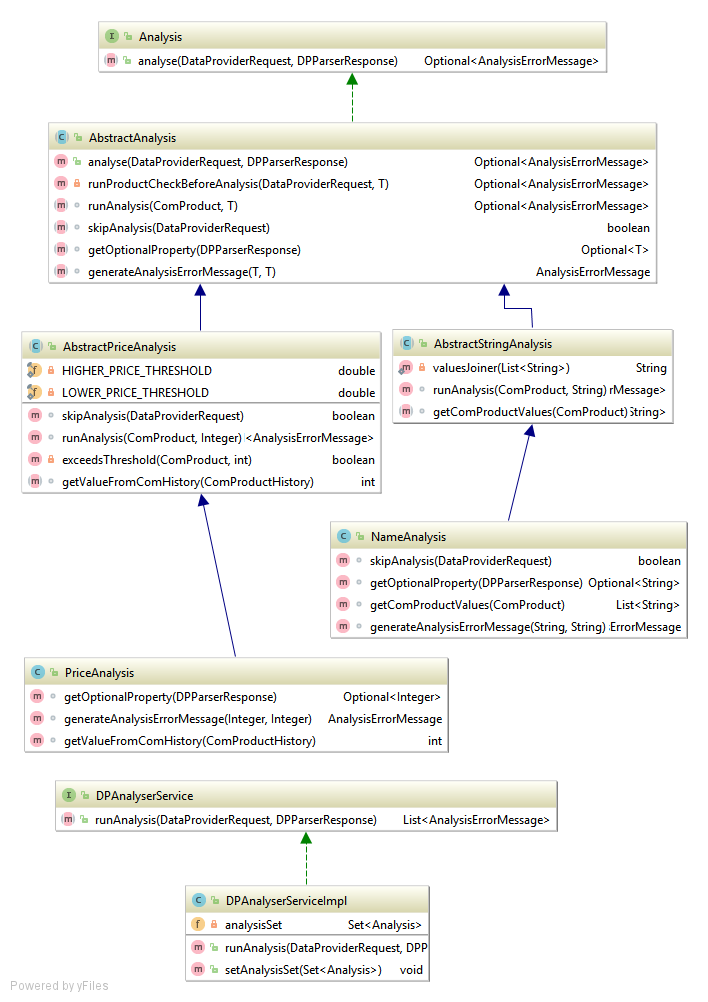
\includegraphics[width=1.0\textwidth]{resources/analyser-classes}
	\caption[Diagram tříd analyzátoru]{Diagra tříd analyzátoru. Obsahuje pouze některé validace pro zachování přehlednosti.}\label{fig:analyser-classes}
\end{figure}


Jak již bylo zmíněno, podobná architektura spouštění validací se vyskytuje na více místech interní části, například u validace po provedení
parsování nebo kontrol, zda má být adresa použita pro vytvoření požadavku.


\section{Plánování práce}\label{ch:planning}
Plánování práce bylo rozděleno do tří částí, nalezení adres, vytvoření požadavků a samotné odeslání.
Tato sekce se týká pouze samotného nalezení adres, které jsou následně použity v dalším zpracování.
\par
V rámci hledání samotných adres byly implementovány servisní třídy, které adresy hledají podle kritérií popsaných v 
návrhu vylepšeních. Následně jsou vráceny v obalovací třídě, která uchovává důvod nalezení adresy. Nalezení adres nově počítá i s frekvencí nastavenou u kampaně.
\par
Nalezené adresy všech typů jsou vyfiltrovány o nežádoucí stavy. K tomuto účelu jsem navrhl rozhraní kontrol, rozhodující 
o tom, zda adresu použít. Tento návrh se podobá validačním kontrolám analyzátoru v modulu DataProvider.

\section{Oprava komunikace Manager - ProductProvider}
Důležitý prvek samotné opravy komunikace modulů Manager a ProductProvider je vytváření požadavků z nalezených adres.
Vzhledem ke změně rozhraní, které zachovává způsob nalezení adres, stačilo vytvořit ostatní části modulu Manager, tak aby odpovídalo novému rozhraní.
\par
Hlavní metoda servisní třídy \textit{DPRequestSenderServiceImpl} volající všechny tří části vypadá následovně:
\begin{lstlisting}[language=Java]
    /**
     * Creates requests and sends them.
     *
     * @throws MQConnectionException when sending fails
     */
    @Override
    public void createRequests() throws MQConnectionException {
        ProductUrlSets requiredProductUrls = prioritizeService.findRequiredProductUrls();

        DPRequestProductUrlWrapper dpRequestWrapper = requestBuilderService.create(
                requiredProductUrls);


        senderService.sendDPRequests(dpRequestWrapper);
    }
\end{lstlisting}
Nejdříve jsou nalezeny adresy, což bylo popsáno v kapitole \ref{ch:planning}. Poté jsou vytvořeny výsledné požadavky
a odeslány. Servisní třída zodpovědná za odeslání zároveň ukládá příznaky stavu do databáze.
\par
Vzhledem v zásadní změně architektury neuvádím původní kód, jelikož celkový způsob vytváření požadavků je značně odlišný a není proto možné jednoduché porovnání. Vytváření bylo v předchozím řešení ve stejné třídě, která zajišťovala i odesílání, což způsobovalo problém při ukládání příznaků do databáze.
\par
Nový návrh vytváření požadavků tento proces deleguje do nové 
třídy  \\ \textit{DPRequestBuilderServiceImpl}, která zajišťuje uložení všech potřebných atributů do nového požadavku. Návratový typ této třídy slučuje skupiny požadavků obsahující adresy bez produktů a ty v aktivní kampani, jelikož nastavení příznaku o chybném odeslání je u obou typů
totožné.
\par
Vzhledem k potřebě pracovat s adresou detailu i při odesílání požadavků, obsahuje \textit{DPRequestProductUrlWrapper} kromě vytvořeného požadavku
i původní adresu detailu produktu. Důvod je možnost přímého přístupu k chybě přes databázovou entitu adresy.

\subsection{Odesílání požadavků}
Odesílání požadavků jsem upravil, aby odpovídalo novému návrhu. Před odesláním je každý požadavek uložen do databáze a nastaven
příznak o zpracování. V případě neočekávané chyby při odesílání, jsou tyto příznaky korektně změněny.
\par
Samotné odeslání má u všech požadavků stejný postup. Nejprve jsem proto extrahoval části obsahující ukládání a změnu stavu požadavků či chyb do samostatné třídy
\textit{DPRequestPersistServiceImpl}. Poté jsem využil nativního rozhraní Java 8, \textit{Consumer<T>}, které reprezentuje
operaci přijímající jeden vstupní parametr a nevrací žádný výsledek. Rozhraní jsem použil k reprezentaci operace uložení a
změny stavu v případě chyby.

\begin{lstlisting}[language=Java, caption={Společná metoda zajišťující odeslání DataProvider požadavků.}]
    /**
     * Sends request via {@link RequestHandler}.
     * Request is first persisted via {@link PersistanceDPRequestFacade} and it's id is set to the request in wrapper
     * object. If failure while sending object through MQ occurs, then {@link Consumer} failureHandler is called,
     * exception logged and rethrown.
     * Package private because of static code analysis.
     *
     * @param requestProductUrl wrapped object containing {@link ProductUrl} and {@link DataProviderRequest}
     * @param persistConsumer   persisting consumer called before sending
     * @param revertConsumer    revert consumer called in case of sending failure
     */
    void send(DPRequestProductUrl requestProductUrl,
              Consumer<DPRequestProductUrl> persistConsumer,
              Consumer<DPRequestProductUrl> revertConsumer) {
        try {
            persistConsumer.accept(requestProductUrl);
            providerRequestHandler.send(
                    requestProductUrl.getDataProviderRequest());
        } catch (MQConnectionException e) {
            revertConsumer.accept(requestProductUrl);
            logger.error("Sending dataProviderRequest error.", e);
            throw new IllegalStateException(e);
        }
    }
\end{lstlisting}

Zde je nutné podotknout důvod, proč není po odchytnutí a zpracování výjimky vrácena opět \textit{MQConnectionException}. 
Zvolený způsob iterace nad objekty a samotného volání odesílací metody totiž neumožňuje obsahovat v těle metodu
vyhazující výjimku rozšiřující třídu \textit{Exception}.
Nedostatek architektury lze obejít pomocí \textit{IllegalStateException}, která potomkem třídy \textit{Exception} není.

\par

\begin{lstlisting}[language=Java, caption={Příklad zavolání metody odesílající požadavky.}]
        dpRequestWrapper.getAnalyserErrors().forEach(x -> send(
                x,
                dpRequestPersistService::persistRequestAnalyserError,
                dpRequestPersistService::revertRequestAnalyserError
                )
        );
\end{lstlisting}

\subsection{Komunikační objekt a využití stažené stránky}
Nejdříve je nutné popsat změnu komunikační třídy \textit{DataProviderRequest}. Tato komunikační třída představuje jeden požadavek odeslaný pomocí front do DataProvider a skládá se z jednotlivých základních atributů a fragmentů.
Fragmentem je myšlena serializovatelná třída představující jeden celek, například informace o produktu nebo šabloně.
\par
Původní návrh počítal s příznakem označující typ požadavku pro DataProvider. Příznak označoval, zda je obsažena stažená stránka či nikoliv. Stav, kdy požadavek obsahoval stránky však nikdy nenastal z důvodu implementace plánování práce a vytváření požadavků. Jelikož jediný rozdíl těchto dvou typů byl v atributu uchovávající staženou stránku, odstranil jsem ho.
\par
Některé další atributy či fragmenty jako produkt nebo šablona nemusejí být nastaveny. U všech těchto atributů a fragmentů jsem proto provedl změnu u \textit{get} metod, aby vracely kontejner \textit{Optional}. Tím je jasně indikovaná možnost, že nemusí být obsaženy.
\par
V rámci DataProvideru stačilo vytvořit při přístupu k jednomu z těchto atributů dvě možné větvení aplikace.
Například pokud byla stránka obsažena v požadavku, třída \textit{DPDownloaderServiceImpl} vrátila validní odpověď o stažení obsahující tuto stránku, což je demonstrováno na následující ukázce.

\begin{lstlisting}[language=Java, caption={Veřejná metoda třídy \textit{DPDownloaderServiceImpl} zajišťující stažení stránky obsahující detail produktu.}]
    /**
     * Downloads requested page and returns {@link DownloaderResponse} object.
     *
     * @param dataProviderRequest the request containing url to be downloaded
     * @return DownloaderResponse encapsulating downloaded data or error
     */
    @Override
    public DownloaderResponse download(DataProviderRequest dataProviderRequest) {
        return dataProviderRequest.getDownloadedPage()
                        .map(x -> new DownloaderResponse(Jsoup.parse(x)))
                        .orElseGet(
                                () -> doDownload(dataProviderRequest)
                        );
    }
\end{lstlisting}


\section{Spojení chyb analyzátoru a vylepšení rozhraní}
Oprava více četnosti chyb a samotného rozhraní je posloupnost několika oprav. 
Bylo již zmíněno odstranění přebytečných výjimek, což zajistilo spouštění všech validací. 
Další krok je změna komunikačního objektu, který nově uchovává všechny chybné validace a detailnější informace
o chybě.
\par
Původní řešení obsahovalo dvě třídy určené pro odpověď, protože DataProvider má dvě výstupní fronty: pro validní odpověď a chybu. 
Třída pro validní odpověď je \textit{DataProviderResponse}, pro chybu pak \textit{DataProviderResponseError}.
\par
Z důvodu velkého množství podobných atributů, obzvlášť po přidání vyparsovaných hodnot do chyby, jsem změnil návrh těchto objektů.
Z \textit{DataProviderResponseError} jsem odstranil společné atributy a jako jeho rodiče jsem zvolil přímo \textit{DataProviderResponse}.
Chybná odpověď nově obsahovala všechny atributy validní odpovědi. 
\par
Z hlediska Managera bylo potřeba tyto hodnoty uložit, jelikož se ukládaly pouze získané ceny. Vytvořil jsem novou tabulku
uchovávající informace o vyparsovaných hodnotách, které mohou být použity v případě zobrazení chyby administrátorovi.
Dále bylo nutné uložit detailní informace o chybách. Proto jsem vytvořil další tabulku, která je spojena vazbou 1:n s databázovou reprezentací chyby.
\par
Dalším krokem bylo upravení webového rozhraní, aby odpovídalo změněné databázové struktuře. První změna se týkala samotného zobrazení
informacích o chybě. Zde jsem využil nově uložených dat. Administrátor má tak možnost vidět použité hodnoty při analyzování a všechny
vyskytnuté chyby. Změna je viditelná na ukázkách webového rozhraní: \ref{fig:analyser-error} a \ref{fig:temp-det-err}.
\par
Poslední úprava spočívala v zpracování vstupů od administrátora, kdy bylo potřeba uložit všechny možné příznaky pro 
budoucí analyzování.

\begin{figure}\centering
 	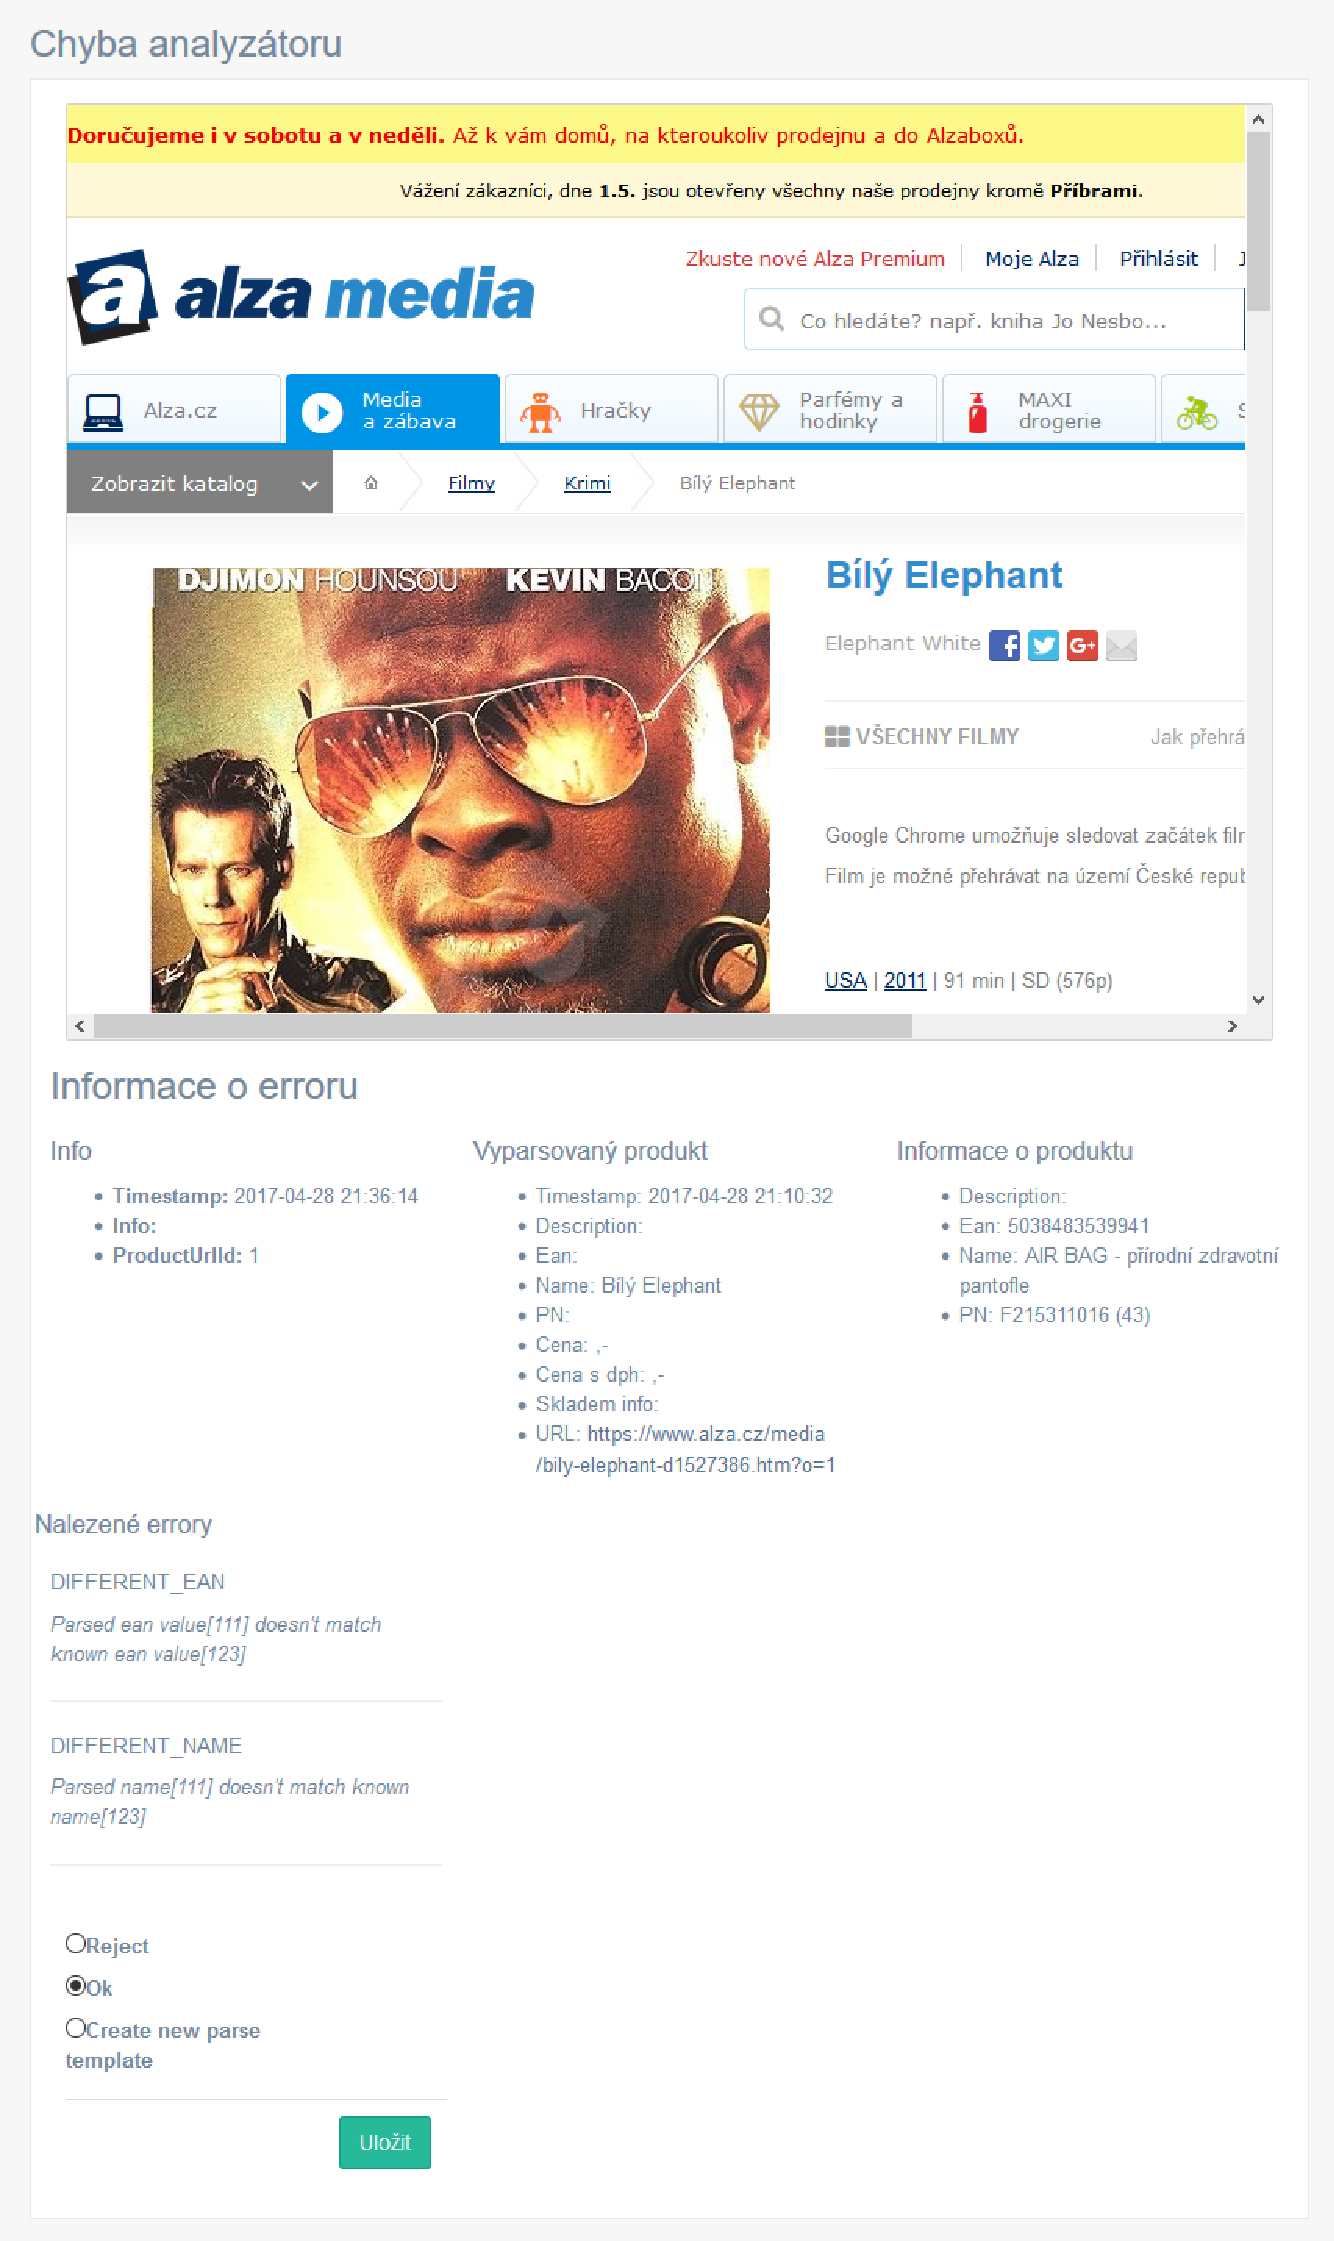
\includegraphics[width=1.0\textwidth]{resources/analyser-err}
	\caption[Webové rozhraní pro vyřešení chyby analyzátoru po provedení vylepšeních]{Ukázka webového rozhraní pro vyřešení chyby analyzátoru po provedení vylepšeních.}\label{fig:analyser-error}
\end{figure}

\section{Monitorování}
Na virtuální server jsem nasadil službu DataDog\cite{dataDog}, která po jednoduché instalaci umožňuje sledování běžících služeb
a vytížení serveru. Data jsou odesílána přímo do služby DataDog. Externí webové rozhraní umožňuje zobrazení posbíraných údajů.
\par
Základní funkcionalita poskytuje pouze informace o využití prostředků a přístup k logům. Ačkoliv základní funkcionalita postačovala pro potřeby 
mého projektu, službu je možné rozšířit o doplňky. Pomocí těch je možné sledovat například výsledek sestavení v Jenkins, ale i obsah a využití RabbitMQ front. 


\section{Získání adres obchodů a příslušných detailů produktů}
Finder byl na základě důvodů popsaných v návrhu rozdělen na dvě části. Část vyhledávající na internetových obchodech adresy detailů popisující diagram aktivit \ref{fig:pdp-diagram} a na část, která samotné obchody vyhledává.
\par
Implementována byla pouze první část, jelikož hledání samotných obchodů lze nahradit manuálním přidání obchodů, na kterých chceme vyhledávat, případně využít některý z veřejných seznamů internetových obchodů v České republice a ty manuálně vložit do databáze.
Jako seznam by bylo možné využít například webovou stránku \href{http://www.i-shopy.cz/}{i-shopy.cz \textit{[cit. 5.5.2017]}}, která indexuje 3091 internetových obchodů.
\par
Modul Finder byl zcela odstraněn a nahrazen modulem novým, nazvaným ProductDetailProvider.
Tento modul zajišťuje hledání adres detailů produktů, což je dosaženo na základě šablony internetového obchodu, která obsahuje 
tyto atributy:
\begin{itemize}
\item formát URL sloužící k vyhledání produktu na obchodě,
\item oddělovač slov v URL adrese,
\item selektory pro výběr adres vedoucí na detaily produktů.
\end{itemize}
Pro vytvoření požadavku je nutná existence šablony, která obsahuje informace, jak na obchodě vyhledávat.
Po nalezení adres je vytvořena chyba pro administrátora, aby specifikoval výběr samotných adres detailů. Webové rozhraní
bylo pro tento proces vytvořeno již v rámci týmového projektu.

\begin{figure}\centering
 	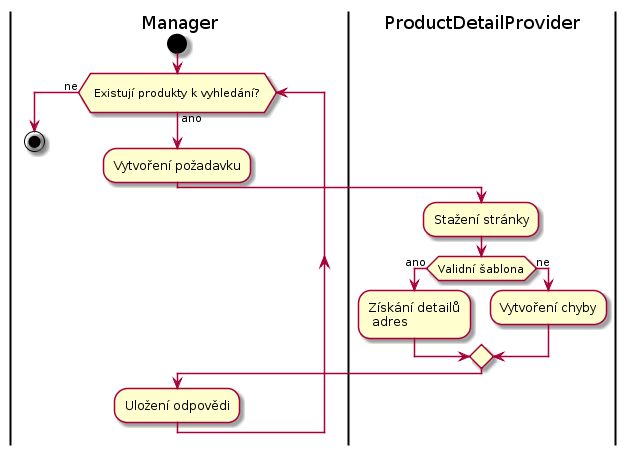
\includegraphics[width=1.0\textwidth]{resources/pdp-activity}
	\caption[Aktivity diagram ilustrující nalezení adres detailů produktů]{
	Aktivity diagram ilustrující nalezení adres detailů produktů.}\label{fig:pdp-diagram}
\end{figure}

\section{Párování produktu}
Byl implementován proces, který se nejprve pokusí produkt spárovat automaticky, pokud nalezne přímou shodu názvu, EANu nebo modelového čísla.
Pro určení shody probíhá porovnání nalezeného identifikátoru s uloženým. Shoda je hledána na základě podřetězců.
\par
Pokud je vyhledání podřetězců neúspěšné, jsou provedeny heuristiky hledající pravděpodobné shody. K detekci shody jsou použity algoritmy počítající společná slova a nejdelší společný podřetězec. Ze všech nalezených možností je vytvořena chyba, kterou musí zpracovat administrátor.
\par 
Do webového části bylo vytvořeno rozhraní, které administrátorovi umožňuje jednoduché přiřazení adresy k produktu nebo všechny nabízené možnosti odmítnout.


\section{Detekce neexistující stránky a nenalezeného produktu}
V případě použití interního vyhledávání se stávalo, že pro hledanou hodnotu nebyl nalezen žádný produkt, což bylo zpracováno
jako chyba šablony, protože struktura stránky definované šabloně neodpovídala. Podobný případ byl u nalezení adresy detailu, která neexistuje, ačkoliv byla vrácena jako výsledek při vyhledávání.I pro tuto možnost byla vytvořena příslušná chyba šablony.
\par
Nejprve jsem se snažil při nenalezení žádných hodnot výsledek porovnat se stránkou, která byla obchodem vrácena při hledání náhodného
řetězce dlouhé délky. Myšlenka byla, že pokud produkt opravdu na obchodu není, stránka vrácena při nesmyslném hledání bude mít podobnou strukturu.
\par
Problémem tohoto řešení se ukázala přílišná odlišnost HTML stažených stránek a specifičnost obchodů. Algoritmus fungoval
pouze na malé části obchodů a proto bylo toto řešení zavrženo.
\par
Nakonec jsem zvolil možnost, kdy administrátor má v rámci řešení chyby šablony možnost zadat řetězec značící neexistenci produktu (popř. neexistující stránky detailu produktu), viz. obrázek \ref{fig:temp-det-err}. Tento řetězec je pro každý obchod specifický a před vytvořením chyby šablony je nejdříve zkontrolováno, zda se řetězec na stránce nenachází. Pokud ano, nejedná se o chybu šablony, ale pouze nebylo nic nalezeno.

\begin{figure}\centering
 	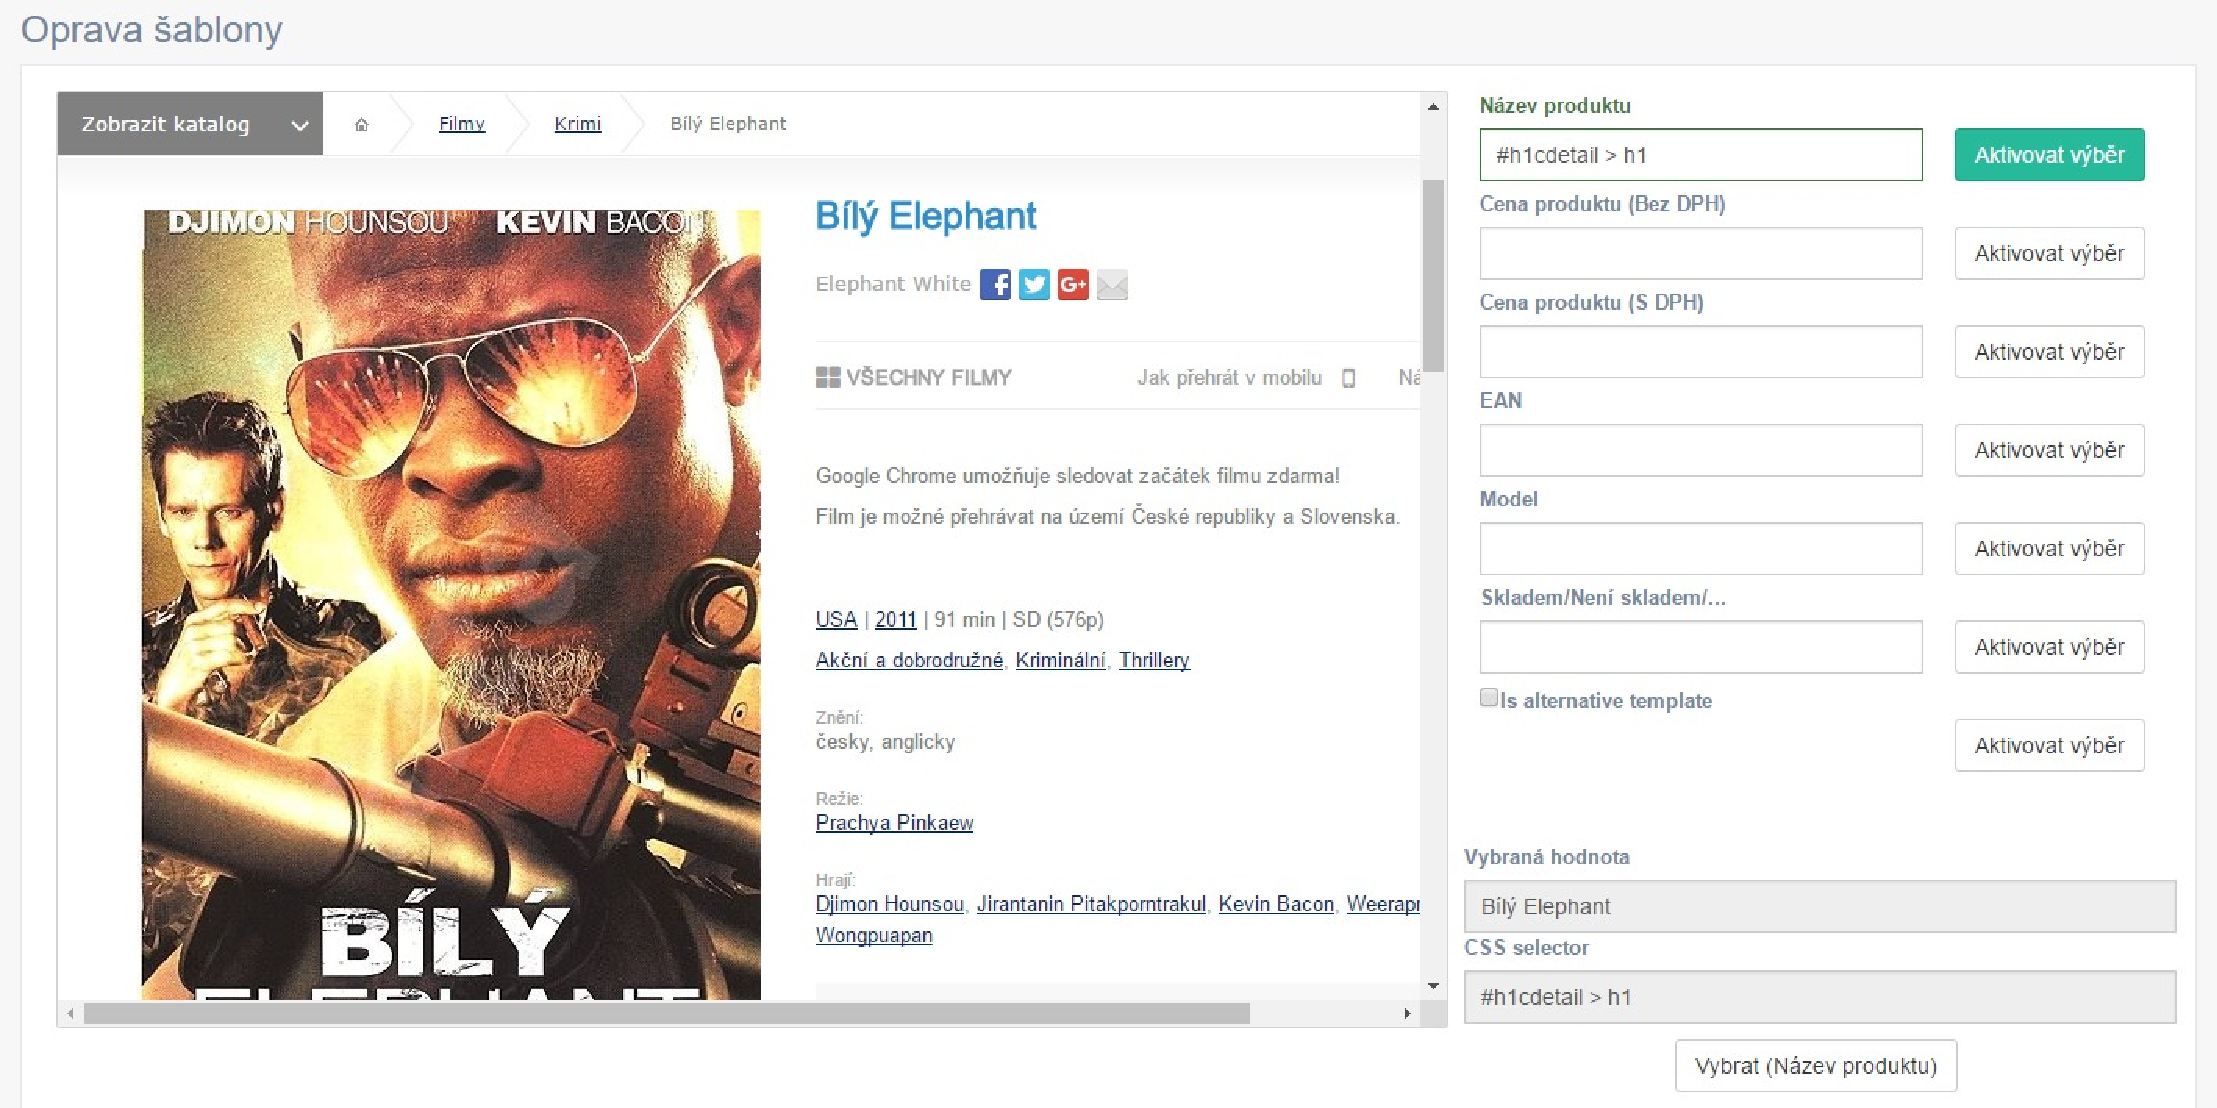
\includegraphics[width=1.0\textwidth]{resources/template-detail-err}
	\caption[Administrátorské rozhraní pro opravu detailu šablony]{Administrátorské rozhraní pro opravu detailu šablony.
	Původní řešení neobsahovalo informaci o použité URL adrese, vyparsované hodnoty a formulář pro chybný řetězec.}\label{fig:temp-det-err}
\end{figure}

\section{Více šablon detailů produktů}
Původní návrh počítal se stavem, kdy stránka detailu produktu  má stejnou strukturu napříč celým obchodem.
Tento předpoklad se při testování ukázal jako chybný, kdy například výskyt slevy způsobil odlišný název elementu.
\par
Důsledek byla chyba šablony. Abych problém odstranil implementoval jsem podporu alternativních šablon, které jsou
použity v případě, že hlavní šablona selže. Možnost uložení šablony jako alternativní jsem zapracoval do běžného rozhraní 
pro editaci šablony detailu.

\section{Více stejných chyb}
Systém se i po změnách potýkal se stavem, kdy se v administrátorském rozhraní objevilo více chyb šablon nebo analyzátoru.
V původním řešení tento stav nastával pokaždé, když byly vytvořeny požadavky pro všechny adresy vedoucí na obchod bez šablony.
\par
Chyby lze predikovat a v případě neexistující šablony odeslat pouze jediný požadavek pro ProductProvider. Ačkoliv jsem 
upravil plánování práce a zároveň přidal kontrolu, která kontroluje zda není takový požadavek již ve frontě, tak se stávalo, že administrátor 
byl v některých případech zahlcen chybami. Zahlcení v tomto způsobovala šablona, která přestala fungovat.
\par
Jelikož tento stav není možné predikovat, zvolil jsem možnost, kdy je pouze upraveno webové rozhraní.
Úprava webového rozhraní spočívala v omezení zobrazování chyb, kdy související chyby jsou v seznamu pouze jednou. 
Změněné zpracování formuláře \uv{vyřešilo} všechny chyby stejného typu, čímž odpadá nutnost je řešit.

\section{Skladem}
V rámci získávání dat u detailu produktu jsem přidal možnost získávat informaci, zda je produkt skladem. Provedl jsem tak na základě
konverzace s provozovatelem internetového obchodu, který tento údaj považuje za důležitý.
\par
Pro úpravu jsem upravil nejdříve rozhraní pro vytváření šablony a strukturu databáze, aby uchovávala atribut u šablony a výsledek parsování.
Zajistil jsem, aby byl tento atribut zahrnut v rámci komunikace modulu Manager a DataProvider, kde bylo potřeba upravit
správné uložení nových atributů do komunikačních tříd, získání hodnoty při parsování a následné uložení do databáze.

\section{Ostatní}
Při realizaci jsem provedl několik menších změn a oprav. Jedna z nich byla například nastavení 
připojení do databáze. Původní stav obsahoval konfiguraci připojení v samostatných \textit{xml} souborech, ve kterých byly zduplikovány
registrace databázových tříd.
\par
Tento způsob jsem přepsal, aby nastavení databázových tříd bylo pouze v jednom souboru. Samotné připojení definují
\textit{properties} soubory, které mají následovnou strukturu:

\begin{lstlisting}[language=Java, caption={Nastavení připojení do databáze.}]
hibernate.hikari.dataSource.url
		=jdbc:mysql://localhost:3306/infoweb-db?characterEncoding=UTF-8
hibernate.hikari.dataSource.user=root
hibernate.hikari.dataSource.password=
hibernate.hikari.dataSourceClassName
	=com.mysql.jdbc.jdbc2.optional.MysqlDataSource
database.dialect=org.hibernate.dialect.MySQL5InnoDBDialect
hibernate.hbm2ddl.auto=create-drop
hibernate.hbm2ddl.import_files=sql/importScript.sql
hibernate.hbm2ddl.import_files_sql_extractor
	=org.hibernate.tool.hbm2ddl.MultipleLinesSqlCommandExtractor
\end{lstlisting}

Úprava pak ulehčuje změny v databázových třídách a umožňuje jednoduchou konfiguraci pro více vývojových prostředí jako například testovací, vývojové
a produkční.


\chapter{Zhodnocení provedených vylepšení}
Zde bych se rád věnoval konečné funkcionalitě systému. Zhodnocení bude provedeno stejným způsobem a podle stejných kriterií jako zhodnocení
týmového projektu, což je podrobně popsáno v sekci \ref{sec:zhodnoceni-typ}. Jediný rozdíl je použití odlišných testovacích dat, což jsem nastínil v předchozí kapitole.


\section{Data}
Testování samotného systému jsem provedl nad reálným vzorkem dat, které mi poskytl provozovatel internetového obchodu.
Data se skládají z údajů o produktech popsaných v tabulce \ref{table:product-test} a internetových obchodů vyjmenovaných v tabulce
\ref{table:product-test-products}.
U každého internetového obchodu bylo v rámci dat zaznamenáno jaké produkty se na něm vyskytují, což mi umožnilo jednoduše kontrolovat, zda systém nalezl všechny adresy detailů.


\begin{table}
\centering
\begin{tabular}{@{}lll@{}}
\textbf{značka} & \textbf{model}   & \textbf{název}                                                                                                  \\ Scholl          & F215311016 (43)  & \begin{tabular}[c]{@{}l@{}}AIR BAG - přírodní\\ zdravotní pantofle\end{tabular}                                 \\ \midrule
Scholl          & F200781065 (43)  & \begin{tabular}[c]{@{}l@{}}CLOG SUPERCOMFORT\\ bílá\end{tabular}                                                \\ \midrule
Scholl          & 4002448095262    & \begin{tabular}[c]{@{}l@{}}Velvet Smooth wet \& dry \\ - elektrický pilník na chodidla do vody\end{tabular}     \\ \midrule
Beurer          & BEU-FB30         & FB 30 nožní masáž                                                                                               \\ \midrule
Sanitas         & SAN-SEM43        & \begin{tabular}[c]{@{}l@{}}SEM 43 svalový a nervový \\ elektrostimulátor\end{tabular}                           \\ \midrule
Beurer          & BEU-464.15       & \begin{tabular}[c]{@{}l@{}}GL 44 / GL 50 / GL 50 EVO\\ testovací proužky 464.15 (2x25ks)\end{tabular}           \\ \midrule
Beurer          & BEU-IPL10000+    & \begin{tabular}[c]{@{}l@{}}IPL 10000+ Depilace SalonPro \\ System - depilace s dlouhodobým účinkem\end{tabular} \\ \midrule
Salter          & SA1008GSBKXR     & SALTER 1008 GSBKXR                                                                                              \\ \midrule
Homedics        & MIR-8150         & MIR M-8150 - kosmetické zrcadlo                                                                                 \\ \midrule
Philips         & Phil-71768/08/16 & Softpal Battery Olaf White                                                                                      \\ \bottomrule
\end{tabular}
\caption{Produkty použité v testovacích datech pro zhodnocení výsledného řešení.}
\label{table:product-test}
\end{table}


\begin{table}
\centering
\begin{tabular}{ | l | l | l |}
\toprule
muj-scholl.cz & kudrnka.cz & 4home.cz \\
muj-beurer.cz & zdravotnickaprodejna.cz & medipharma.cz \\
muj-sanitas.cz & eobuv.cz & obuv-scholl.cz \\
muj-salter.cz & mall.cz & k24.cz \\
muj-homedics.cz & pilulka.cz & alza.cz \\
elektrocr.cz & expert.cz & cesky-obchodak.eu \\
ajtrade.cz & datart.cz & diagnosticketesty.cz \\
nakupka.cz & & \\ \bottomrule
\end{tabular}
\caption{Obchody použité v testovacích datech pro zhodnocení výsledného řešení.}
\label{table:product-test-products}
\end{table}

\section{Funkcionalita}
Díky implementaci požadované funkcionality a oprav kritických chyb, je v upraveném řešení možné využít celý proces hledání informací.
Administrátor nově musí zadat přes webové rozhraní obchody, na kterých chceme hledat. Po vytvoření kampaně je také nutné nastavit příslušné šablony 
a spárovat produkty, kde to nebylo možné provést automaticky.

\newpage

\section{Dodatečné opravy}
Plynulost a funkčnost celého procesu hledání dat byla dosažena pouze díky opravám chyb, které jsem nalezl v průběhu testování.
V kapitole Realizace vylepšení \ref{ch:realisation} jsem popisoval implementaci dodatečných oprav. Je však nutné zmínit, jak byly tyto nedostatky nalezeny.

\subsection{Více šablon detailů produktu a Více stejných chyb}
Chyba, kdy obchod obsahoval více možných struktur pro detaily produktů a zobrazení více stejných chyb ve webovém rozhraní měly stejnou příčinu.
\par
Systém při vyhledávání na obchodech \textit{alza.cz} a \textit{nakupka.cz} nalezl detaily produktů, které měly jinou strukturu než uložená šablona.
Výsledek byla neočekávaná chyba, což způsobilo více stejných chyb. Chyby zahlcovaly webové rozhraní. Oprava rozhraní ovšem neřešila
problém odlišné struktury a proto bylo třeba vytvořit i podporu pro šablony alternativní.
\subsection{Neexistující stránka}
Neúspěšné vyhledávání se vykytovalo na většině obchodech, protože hledaný produkt se na stránkách nenacházel. Systém prázdnou stránku detekoval jako chybu šablony.
\par
Neexistující stránka detailu pak byla objevena na obchodě kudrnka.cz, kdy interní vyhledávání vracelo odkaz na neexistující detail produktu, což opět způsobilo chybu šablony, jelikož nebyla vyparsována žádná hodnota.

\section{Párování}
Při testování bylo zjištěno, že velké množství obchodů neobsahuje správné nebo přímo odlišné identifikátory produktů. Nejčastější je výskyt pouze jména, které často neodpovídá tomu uloženému.
\par
Obchody poskytující pouze název znamenají nutnost provést párování manuálně. Systém se párování snaží ulehčit rozhraním, nicméně i při malém množstvím produktů je celkový počet těchto chyb velmi rozsáhlý. 
\par
Například na obchodě \textit{mall.cz} bylo nutné manuálně spárovat 4 ze 6 produktů. Počet všech nabízených možností párování pro administrátora bylo 30. Jeden produkt se na obchodě nepodařilo nalézt a spárovat vůbec, jelikož obsahoval kompletně odlišný název oproti uloženému.
\par
Proces párování by bylo možné vylepšit, pokud by systém uchovával více identifikátorů. Více uložených jmen by pak zátěž na administrátora mohla s časem klesnout, protože použitých jmen napříč obchody je omezené množství.
U kompletně odlišných názvů je jediné řešení, vytvoření rozhraní umožňující čistě manuální párování.

\section{Webové rozhraní}\label{ch:web-interface}
Nalezl jsem nedostatky ve webovém rozhraní, kdy jeho funkčnost sloužící k opravám šablony detailu, nebyla na některých obchodech funkční.
Jednalo se například o obchod \textit{pilulka.cz}, kde se při zobrazení staženého HTML nezobrazoval EAN, takže nebylo možné nastavit příslušný selektor. 
U obchodu \textit{mall.cz} byl pro změnu obsah stránky překryt upozorněním o nepodporovaném prohlížeči.
\par
Problém obsahovala i část pro šablonu sloužící k nalezení adres detailů. Pokud bylo použito rozhraní, šablona nebyla ve většině
případů funkční. 
\par
Chyby v obou částech nejsou kritické, jelikož při zadání cesty k elementu manuálně, uložení šablony proběhne správně a systém může pokračovat
v práci.

\section{Návrh a testy}
Zásadní refaktoring a změna návrhu komunikace tříd velmi pozměnila interní část. 
Interní část vyhovuje nárokům na formu. Je složena z přehlednějšího, udržovatelnějšího a
lépe rozšiřitelného kódu.
\par
Tyto vlastnosti byly výrazné při úpravách, kdy změny byly často triviální záležitost.
Kromě subjektivního pocitu rychlejší orientace v kódu, nová architektura umožnila jednoduché přidání vylepšení
a po provedení bylo zachována původní funkcionalita. Toto dávám za důsledek lepšímu pokrytí
testy a rozdělení tříd do menších celků. Oproti původnímu řešení narostl počet jednotkových
testů ze 170 na 492. Pokrytí v procentech demonstruje následující vizualizace.

\begin{figure}[h]\centering
 	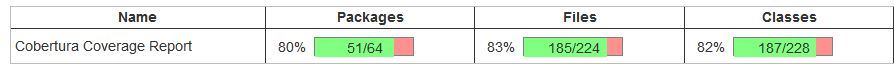
\includegraphics[width=1.0\textwidth]{resources/cobertura-report-new-1}
 	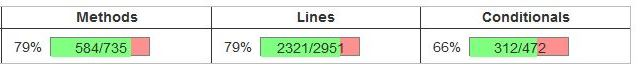
\includegraphics[width=0.7\textwidth]{resources/cobertura-report-new-2}
	\caption[Pokrytí testy po provedených vylepšení]{Pokrytí testy po provedených vylepšení. Získáno pomocí nástroje Cobertura. Vizualizace
	výsledků byla vytvořena při sestavení na Jenkins s příslušným doplňkem.}\label{fig:cober-new}
\end{figure}

Pokrytí vzrostlo zhruba o 20\%. Základní funkcionalita servisních tříd je testy pokrytá celá.
Neotestované části jsou především větve, která nastanou při neočekávané chybě a vyhození výjimky, kterou není možné jednoduše v testech nasimulovat.
Další neotestované třídy se týkají komunikace s frontami a jednoduchých objektů, které vrací v \textit{get} metodě \textit{Optional}, což je detekováno jako neotestovaný řádek.
\par
Po provedení změn zůstala nemožnost vytvoření více instancí jednotlivých modulů, tedy ProductDetailProvider a DataProvider.
Pro změnu však stačí přidat instanční rozhraní do jednotlivých modulů, jelikož momentálně jsou spouštěny přímo modulem Manager. Oddělení neovlivní samotnou komunikaci jednotlivých části, nicméně vzroste zátěž na nastavení infrastruktury a nasazení aplikace na server.

\section{Rozhraní administrátora}
Systém se stal z hlediska pro administrátora uživatelsky přívětivější. Při řešení chyb je rozhraní přehlednější a informace o chybách
obsáhlejší. Dále byla snížena zátěž na administrátora, jelikož odpadla nutnost řešit
všechny požadavky týkající se stejného obchodu či chyb analyzátoru.
\par 
Nevýhodou jsou nedostatky týkající se vytváření šablon, které byly zmíněny v kapitole \ref{ch:web-interface}.

\section{Nemožnost vyhledávání na některých obchodech}
V rámci testování jsem objevil nemožnost vyhledávat na obchodech, které mají vyhledávání implementované pomocí POST požadavku, což
systém aktuálně nepodporuje. Jedná se například o obchod \textit{elektrocr.cz}.

\section{Shrnutí}

\begin{table}[h]\centering
    \begin{tabular}{ | l | p{7cm} |}
    \hline
    Typ & Popis \\ \hline
    Kritické chyby & 
  		 \\ \hline
	\hline
    Úplnost funkcionality & 
    	\begin{itemize}
  			\item Systém nevyhledává internetové obchody.
  			\item Nemožnost vyhledávat na některých obchodech.
  		\end{itemize} \\ \hline
	\hline
	Rozšiřitelnost  & 
		\begin{itemize}
  			\item Návrh se ukázal jako vhodný pro úpravy.
  			\item 80 \% pokrytí testy dle nástroje Cobertura.
  			\item 0 chyb statické analýzy kódu.
  		\end{itemize} \\ \hline
    \end{tabular}
	\caption{První část přehledu nedostatků po implementaci navržených vylepšení.}
	  \label{table:analysis-new1}
\end{table}
\begin{table}[h]\centering
    \begin{tabular}{ | l | p{7cm} |}  
    \hline
    Typ & Popis \\ \hline
	Neefektivní chování & 
	 \\ \hline	
	\hline
	Uživatelská přívětivost & 
		\begin{itemize}
  			\item Velká náročnost párování detailů adres s produkty.
  			\item Rozhraní pro editace šablony detailu není funkční na některých stránkách.
  			\item Nefunkční rozhraní pro editaci šablony pro vyhledávání na obchodě.
  		\end{itemize} \\ \hline	
	\hline
	Škálovatelnost & 
		\begin{itemize}
  			\item Nemožnost vytvořit více instancí modulů.
  		\end{itemize} \\ \hline
    \end{tabular}
	\caption{Druhá část přehledu nedostatků po implementaci navržených vylepšení.}
	\label{table:analysis-new2}
\end{table}


\chapter{Závěr}
Vytvořené řešení týmového projektu nevyhovovalo požadavkům na funkcionalitu a možnostem na budoucí rozvoj.
Funkcionalita nebyla splněna především z důvodu nezapojení části, která má za úkol hledat samotné obchody a adresy detailů produktů, které obsahují
hledaná data. Nebyl také vyřešen proces párování produktu k adrese. Návrh některých tříd se ukázal jako nevhodný pro budoucí rozšíření.
\par
V návaznosti na tyto nedostatky bylo navrženo rozsáhlé refaktorování, změna architektury problémových tříd a opravení stávajících
procesů. Bylo potřeba opravit procesy, které nebyly funkční, ztěžovaly práci administrátora nebo byly neefektivní. U funkcionality, kterou měla zajišťovat nezapojená část bylo rozhodnuto o jejím rozdělení, kdy
podpora hledání samotných obchodů byla nahrazena manuálním vložením přes webové rozhraní.
\par
Refaktorování a změna návrhu tříd potvrdila, že se jedná do budoucna o výhodný krok zajišťující lepší udržovatelnost a rozšiřitelnost kódu. Což se ukázalo už při následných změnách, které bylo možné provést v rámci vytvořeného návrhu.
Oprava stávajících procesů pak byla nejvíce viditelná v lepší uživatelské přivětivosti pro administrátora umožňují
případné problémy řešit rychleji a spolehlivěji.
\par
Po implementaci hledání detailu produktu na stránkách obchodů a procesu párování produktů s nalezenými adresami byly
objevené nové nedostatky.
\par
Kritické problémy opravila nová implementace, ale ukázalo se, že i po provedení změn není možné systém použít pro provoz, kde
je požadavek na univerzalitu systému. Systém je po správném nastavení schopný dlouhodobě a automaticky sbírat určitý vzorek dat. Byly však objeveny obchody, kde to není možné. Důvod je především odlišná funkcionalita vyhledávání produktů na sledovaných obchodech, kterou vytvořený systém aktuálně nepodporuje.
\par
Ačkoliv v závěru objevené nedostatky způsobují diskomfort při používání, věřím že přidání funkcionalit navržených v 7. kapitole, umožní plnohodnotné použití výsledného systému.

\bibliographystyle{csn690}



\bibliography{mybibliografy}

\appendix

\chapter{Seznam pojmů}

\section{Web API}
Web Aplication Programming Interface je rozhraní, které na definovaný HTTP dotaz vrátí požadované data. Data jsou standardně vracena ve formátech JSON nebo XML.

\section{Verzovací systém Git}
Git\cite{GIT} je verzovací systém umožňující vytváření a sdílení jednotlivých verzí projektu.
Umožňuje jednoduchý přehled nad rozpracovanými částmi každého vývojáře. Úložiště systému se nazývá repozitář, který obsahuje veškerý kód.
\par
Repozitář existuje v lokálních verzi a zároveň serverové, tedy sdílené. Sdílený repozitář zajišťuje distribuci aktuální verze do lokálních 
repozitářů. Pro lepší správu existují nadstavby nad serverovou částí repozitáře, které umožňují jednoduchou
správu nad kódem a spouštění dalších služeb v závislosti na změnách v kódu.
\par
Základní jednotku tvoří verze, které jsou postupně vytvářeny vývojáři na základě provedených změn.
Verze jsou uchovávány v jednotlivých větvích programu. 
\par
Repozitář je obvykle rozdělen na hlavní a vedlejší větve. Vedlejší větve slouží pro samotný vývoj. 
Hlavní větve tento kód spojují a reprezentují aktuální vývojovou a produkční verzi. Git také obsahuje nástroj pro slučování větví.

\begin{figure}[h]\centering
 	
\includegraphics[width=0.7\textwidth]{resources/branches}
	\caption[Větve v Git repozitáři]{Zobrazení větví v repozitáři, kde \textit{master} je produkční, \textit{develop} vývojová a \textit{topic}
	představuje větev vedlejší}\label{fig:vetev}
\end{figure}

\section{Jednotkové a integrační testy}
Jednotkovými testy se rozumí sada kladných a záporných testů ověřující funkcionalitu jediné třídy. Jednotkové testy
jsou nezávislé na ostatních třídách a testech.\cite{testing} 
\par
Integrační testy pokrývají komunikaci více tříd nebo komunikaci s operačním systémem, hardwarem či rozhraním různých systémů.\cite{testing}
\par
Důvody pro psaní testů jsou například jednodušší nalezení chyby nebo lepší udržovatelnost projektu. V případě neexistujících testů nelze ověřit původní
funkcionalitu při modifikaci aplikace, což může způsobit nutnost nejprve chyby před opravou nalézt.\cite{testing}

\section{Statická analýza kódu}
Statická analýza kódu je analýza softwarového produktu, která běží bez spuštění samotné aplikace. Kontroluje 
pouze kód. Označuje kritické konstrukce vedoucí k chybám nebo nedodržení programátorských konvencí daného
jazyka.
\section{Průběžná integrace}
Průběžnou integrací se rozumí sada nástrojů sloužící k urychlení softwarového vývoje. Základem je průběžné sestavení
a spouštění testů aplikace na základě změn ve sdíleném repozitáři. Lze tak rychle odhalit případné chyby před zařazením 
příslušné verze do produkce.\cite{CI}

\section{Sdílení dat pomocí front}
Sdílení dat pomocí front funguje na principu odesílání zpráv reprezentující objekty. Zprávy jsou po zařazení producentem do fronty odebírány
konzumenty, které je zpracovávají.
Příklad implementace takového systému pak může být RabbitMQ.\cite{rabbitMQ}

\section{JSON}
JSON označuje specifikaci formátu pro výměnu dat\cite{JSON}. Jedná se o formát, který je čitelný nejenom pro lidské oko, ale i pro stroj\cite{JSON},
Zpracování toho formátu je implementováno pro většinu programovacích jazyků\cite{JSON-impl}. Skládá se z párů označující
klíč a hodnotu. Hodnota může být řetězec, číslo nebo pole. Pole pak může uchovávat opět pole, řetězec nebo číslo.\cite{JSON}

\begin{lstlisting}[language=JavaScript, caption={Ukázka formátu JSON}]
{
  "key": [
    1,
    2,
    3
  ],
  "boolean": true,
  "null": null,
  "number": 123,
  "object": {
    "a": "b",
    "c": "d",
    "e": "f"
  },
  "string": "Hello World"
}
\end{lstlisting}

\section{Mock}
V objektově orientovaném programování se Mock objekt používá pro simulování chování konkrétní třídy.\cite{mock}
Při testování je tak možné docílit takových testů, které nejsou závislé na ostatních třídách, kromě té přímo testované.
\par
Testovaná třída obvykle vyžaduje závislost na jiných třídách či rozhraní. Pomocí Mocku je možné chování těchto tříd simulovat.
Mimo nadefinování požadovaného chování, lze také na Mock objektu sledovat jaká na něm byla provedena volání, včetně toho
s jakými parametry. Díky tomu je možné testovat i vnitřní chování testované třídy a ne pouze návratovou hodnotu na základě 
obdrženého vstupu.\cite{mock}

\section{Refaktorování kódu}
Refaktorování v softwarovém vývoji chápeme jako proces restrukturalizace existující kódu, aniž by byla 
pozměněna funkcionalita. Provádí se za účelem dosáhnout průhlednějšího a čitelnějšího kódu, který
se lépe udržuje a rozšiřuje.\cite{refaktoring} Hlavní spouštěcí příčina refaktorování kódu je však existence 
konstrukcí značící špatný návrh aplikace. 

V kontextu této práce jsou důležité především následující konstrukce značící možné problémy\cite{refaktoring}:  
\begin{itemize}
\item Dlouhá metoda.
\item Velká třída.
\item Dlouhý seznam parametrů.
\item Složité struktury podmínek.
\end{itemize}

\chapter{Seznam použitých zkratek}
% \printglossaries
\begin{description}
	\item[EAN] European Article Number,
	\item[XML] Extensible markup language,
	\item[HTML] Hypertext Markup Language,
	\item[CSS] Cascading style sheets,
	\item[JSON] JavaScript Object Notation,
	\item[HTTP] Hypertext Transfer Protocol,
	\item[DAO] Data Access Object,
	\item[URL] Uniform Resource Locator.

\end{description}

\chapter{Obsah přiloženého CD}

%upravte podle skutecnosti

\begin{figure}
	\dirtree{%
		.1 readme.txt\DTcomment{stručný popis obsahu CD}.
		.1 build\DTcomment{adresář se sestavenými verzemi systému}.
		.2 backend\DTcomment{adresář obsahující sestavenou interní část}.
		.2 backend-old\DTcomment{adresář obsahující ses. interní část původního řešení}.
		.1 docs\DTcomment{dokumentace systémuom}.
		.2 backend\DTcomment{dokumentace interní částí}.
		.2 frontend\DTcomment{dokumentace webového rozhraní}.
		.1 src\DTcomment{zdrojové kódy implementace}.
		.2 backend\DTcomment{zdrojové kódy interní částí}.
		.2 backend-old\DTcomment{zdrojové kódy interní částí původního řešení}.
		.2 frontend\DTcomment{zdrojové kódy webového rozhraní}.
		.2 frontend-old\DTcomment{zdrojové kódy webového rozhraní původního řešení}.
		.1 text\DTcomment{zdrojová forma práce ve formátu \LaTeX{}}.
		.2 thesis.pdf\DTcomment{text práce ve formátu PDF}.
	}
\end{figure}

\end{document}
